\documentclass[aspectratio=169]{beamer}

% ---- Packages ----------------------------------------------------------------
\usepackage[T1]{fontenc}
\usepackage[utf8]{inputenc}
\usepackage{amsmath,amssymb}
\usepackage{booktabs}
\usepackage{tikz}
\usetikzlibrary{arrows.meta,positioning,shapes.geometric,backgrounds,fit}
\usepackage{xcolor}
\usepackage{graphicx}
\usepackage{hyperref}
\usepackage{microtype}
\usepackage{xmpmulti}
\usepackage{pgfplots}
\pgfplotsset{compat=newest}
\usepackage{siunitx}
\usepackage{longtable}
\sisetup{round-mode=places,round-precision=1}
\usepackage{braket}
\usetikzlibrary{arrows.meta, shapes.misc, positioning, backgrounds}
\usetikzlibrary{calc, decorations.markings,decorations.pathmorphing}




% ---- Colour palette ----------------------------------------------------------
\definecolor{mqblue}{RGB}{0,73,135}       % deep institute blue
\definecolor{mqgold}{RGB}{200,155,40}     % warm gold accent
\definecolor{mqlight}{RGB}{220,232,245}   % very light blue tint
\definecolor{mqmid}{RGB}{90,140,195}      % mid blue for accents
\definecolor{mqgray}{RGB}{80,80,80}       % body text gray
\definecolor{mqalert}{RGB}{180,40,40}     % red for emphasis

% ---- Beamer theme ------------------------------------------------------------
\usetheme{default}
\usecolortheme{default}
\usefonttheme{professionalfonts}

\setbeamercolor{frametitle}{fg=white,bg=mqblue}
\setbeamercolor{title}{fg=white}
\setbeamercolor{subtitle}{fg=mqgold}
\setbeamercolor{author}{fg=mqlight}
\setbeamercolor{date}{fg=mqlight}
\setbeamercolor{normal text}{fg=mqgray}
\setbeamercolor{structure}{fg=mqblue}
\setbeamercolor{alerted text}{fg=mqalert}
\setbeamercolor{block title}{fg=white,bg=mqblue}
\setbeamercolor{block body}{fg=mqgray,bg=mqlight}
\setbeamercolor{itemize item}{fg=mqgold}
\setbeamercolor{itemize subitem}{fg=mqmid}
\setbeamercolor{enumerate item}{fg=mqblue}
\setbeamercolor{footline}{fg=white,bg=mqblue}

% ---- Title page background ---------------------------------------------------
\setbeamercolor{background canvas}{bg=white}

% ---- Frametitle style --------------------------------------------------------
\setbeamertemplate{frametitle}{%
  \vspace{0.05cm}%
  \begin{beamercolorbox}[wd=\paperwidth,ht=0.65cm,dp=0.2cm,leftskip=0.4cm]{frametitle}%
    \usebeamerfont{frametitle}\insertframetitle%
    \ifx\insertframesubtitle\empty\else%
      \\\usebeamerfont{framesubtitle}\textcolor{mqgold}{\insertframesubtitle}%
    \fi%
  \end{beamercolorbox}%
}

% ---- Footline ----------------------------------------------------------------
\setbeamertemplate{footline}{%
  \begin{beamercolorbox}[wd=\paperwidth,ht=0.42cm,dp=0.15cm]{footline}%
    \hspace{0.4cm}%
    \textcolor{mqlight}{\footnotesize AI \& Quantum Technologies}%
    \hfill%
    \textcolor{mqlight}{\footnotesize M.~Hjorth-Jensen \quad}%
    \textcolor{mqgold}{\footnotesize\insertframenumber\,/\,\inserttotalframenumber}%
    \hspace{0.3cm}%
  \end{beamercolorbox}%
}

% ---- Navigation symbols off --------------------------------------------------
\setbeamertemplate{navigation symbols}{}

% ---- Itemize bullets ---------------------------------------------------------
\setbeamertemplate{itemize item}{\raisebox{0.15ex}{\small$\blacktriangleright$}}
\setbeamertemplate{itemize subitem}{\raisebox{0.15ex}{\small$\triangleright$}}

% ---- Font sizes --------------------------------------------------------------
\setbeamerfont{frametitle}{size=\large,series=\bfseries}
\setbeamerfont{framesubtitle}{size=\normalsize,series=\mdseries}
\setbeamerfont{title}{size=\LARGE,series=\bfseries}
\setbeamerfont{subtitle}{size=\large,series=\mdseries}
\setbeamerfont{block title}{size=\normalsize,series=\bfseries}

% ---- Convenience command: highlighted box ------------------------------------
\newcommand{\hlbox}[2][mqlight]{%
  \begin{beamercolorbox}[rounded=true,shadow=false,sep=4pt,wd=\linewidth]{block body}%
    \textcolor{mqblue}{\small #2}%
  \end{beamercolorbox}%
}

% ---- Title block colours for the title page ----------------------------------
\setbeamertemplate{title page}{%
  \begin{tikzpicture}[remember picture, overlay]
    % Full blue background
    \fill[mqblue] (current page.south west) rectangle (current page.north east);
    % Gold accent bar at top
    \fill[mqgold] ([yshift=-0.0cm]current page.north west)
                  rectangle ([yshift=-0.18cm]current page.north east);
    % Decorative diagonal stripe (subtle)
    \fill[mqmid,opacity=0.25]
      ([xshift=8cm,yshift=0cm]current page.south west)
      -- ([xshift=16.5cm,yshift=0cm]current page.south west)
      -- (current page.north east)
      -- ([xshift=10cm]current page.north east)
      -- cycle;
    % Gold bar at bottom
    \fill[mqgold] ([yshift=0.55cm]current page.south west)
                  rectangle (current page.south east);
  \end{tikzpicture}%
  \vspace{1.4cm}%
  \begin{center}%
    {\usebeamerfont{title}\usebeamercolor[fg]{title}\inserttitle\par}%
    \vspace{0.5cm}%
    {\usebeamerfont{subtitle}\textcolor{mqgold}{\insertsubtitle}\par}%
    \vspace{0.8cm}%
    \textcolor{white!80!mqblue}{\large\insertauthor}\par%
    \vspace{0.25cm}%
    \textcolor{white!60!mqblue}{\normalsize\insertinstitute}\par%
    \vspace{0.25cm}%
    \textcolor{mqgold}{\small\insertdate}%
  \end{center}%
}

% =============================================================================
\title{AI and Quantum Technologies}
\author{Morten Hjorth-Jensen}
\institute{Department of Physics and Center for Computing in Science Education, University of Oslo, Norway}
\date{CircleU Frontiers in Artificial Intelligence, April 15, 2026 }
% =============================================================================

\begin{document}

% ---- Title slide -------------------------------------------------------------
\begin{frame}[plain]
  \titlepage
\end{frame}

% ---- Outline -----------------------------------------------------------------
\begin{frame}{Outline}
\tableofcontents
\end{frame}

\section{A kind of Introduction}


\begin{frame}[plain,fragile]
\frametitle{From Moore's law to Huang's law, the race for more performance}

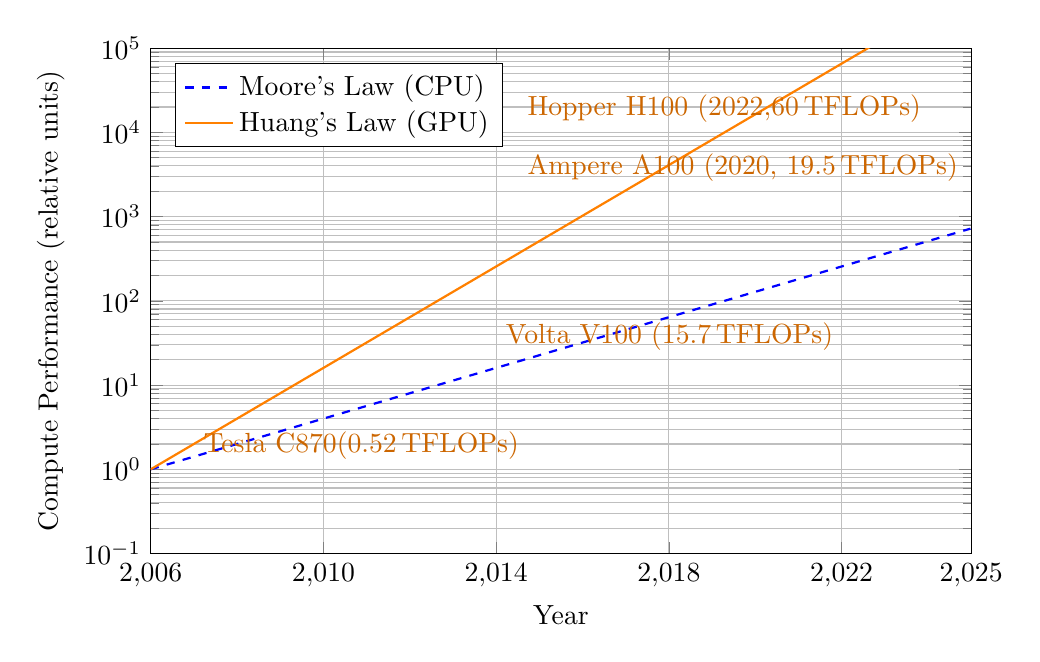
\begin{tikzpicture}
  \begin{semilogyaxis}[
    width=12cm, height=8cm,
    xlabel={Year},
    ylabel={Compute Performance (relative units)},
    xmin=2006, xmax=2025,
    ymin=0.1, ymax=1e5,
    xtick={2006,2010,2014,2018,2022,2025},
    grid=both,
    legend pos=north west,
    legend cell align=left,
    every axis plot/.append style={thick}
  ]

  % Moore's Law (doubling every two years)
  \addplot[
    blue, dashed, domain=2006:2025, samples=200
  ] {2^((x-2006)/2)};
  \addlegendentry{Moore's Law (CPU)}

  % Huang's Law (doubling every year)
  \addplot[
    orange, domain=2006:2025, samples=200
  ] {2^(x-2006)};
  \addlegendentry{Huang's Law (GPU)}

  % GPU Milestones
  \node[anchor=south west,orange!80!black] at (axis cs:2007,1) {Tesla C870(\SI{0.52}{TFLOPs})};
  \node[anchor=south west,orange!80!black] at (axis cs:2014,20) {Volta V100 (\SI{15.7}{TFLOPs})};
  \node[anchor=south west,orange!80!black] at (axis cs:2014.5,2000) {Ampere A100 (2020, \SI{19.5}{TFLOPs})};
  \node[anchor=south west,orange!80!black] at (axis cs:2014.5,10000) {Hopper H100 (2022,\SI{60}{TFLOPs})};
  \end{semilogyaxis}
\end{tikzpicture}

\end{frame}



\begin{frame}[plain,fragile]
\frametitle{Machine learning and AI models are computationally expensive}


% inline figure
\centerline{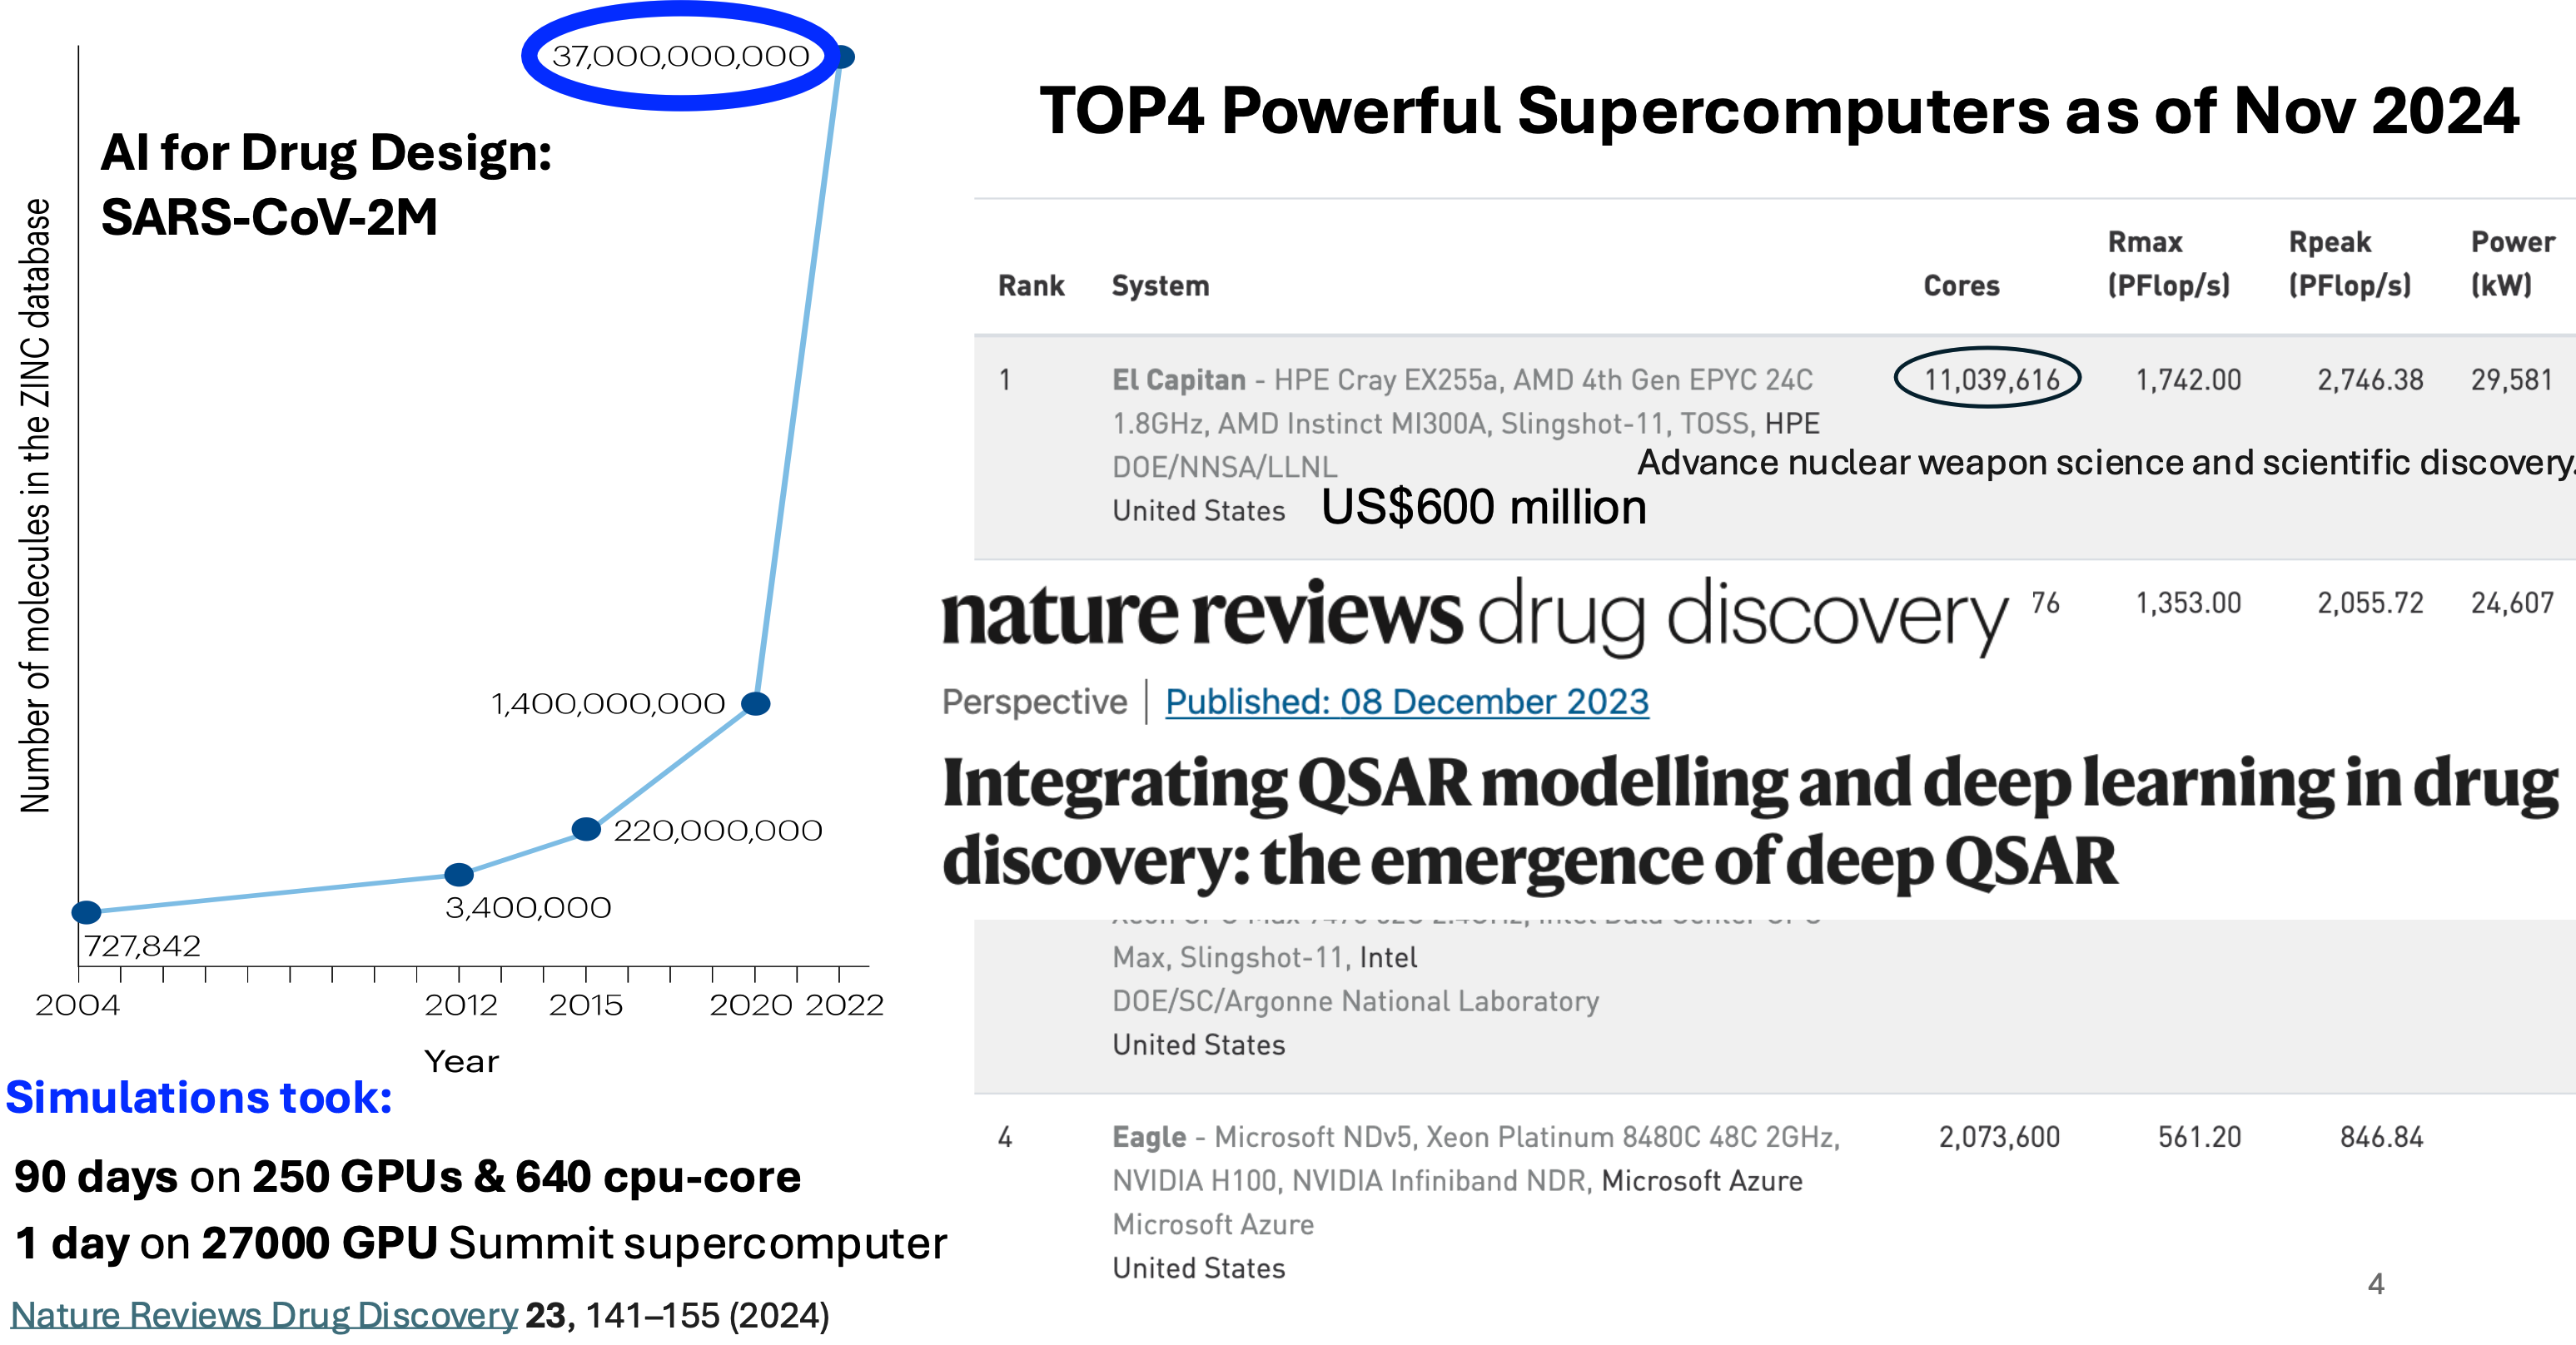
\includegraphics[width=1.0\linewidth]{figures/aitalk2.png}}

\end{frame}


\begin{frame}[plain,fragile]
\frametitle{And power greedy, perhaps quantum computers can reduce the impact?}

% inline figure
\centerline{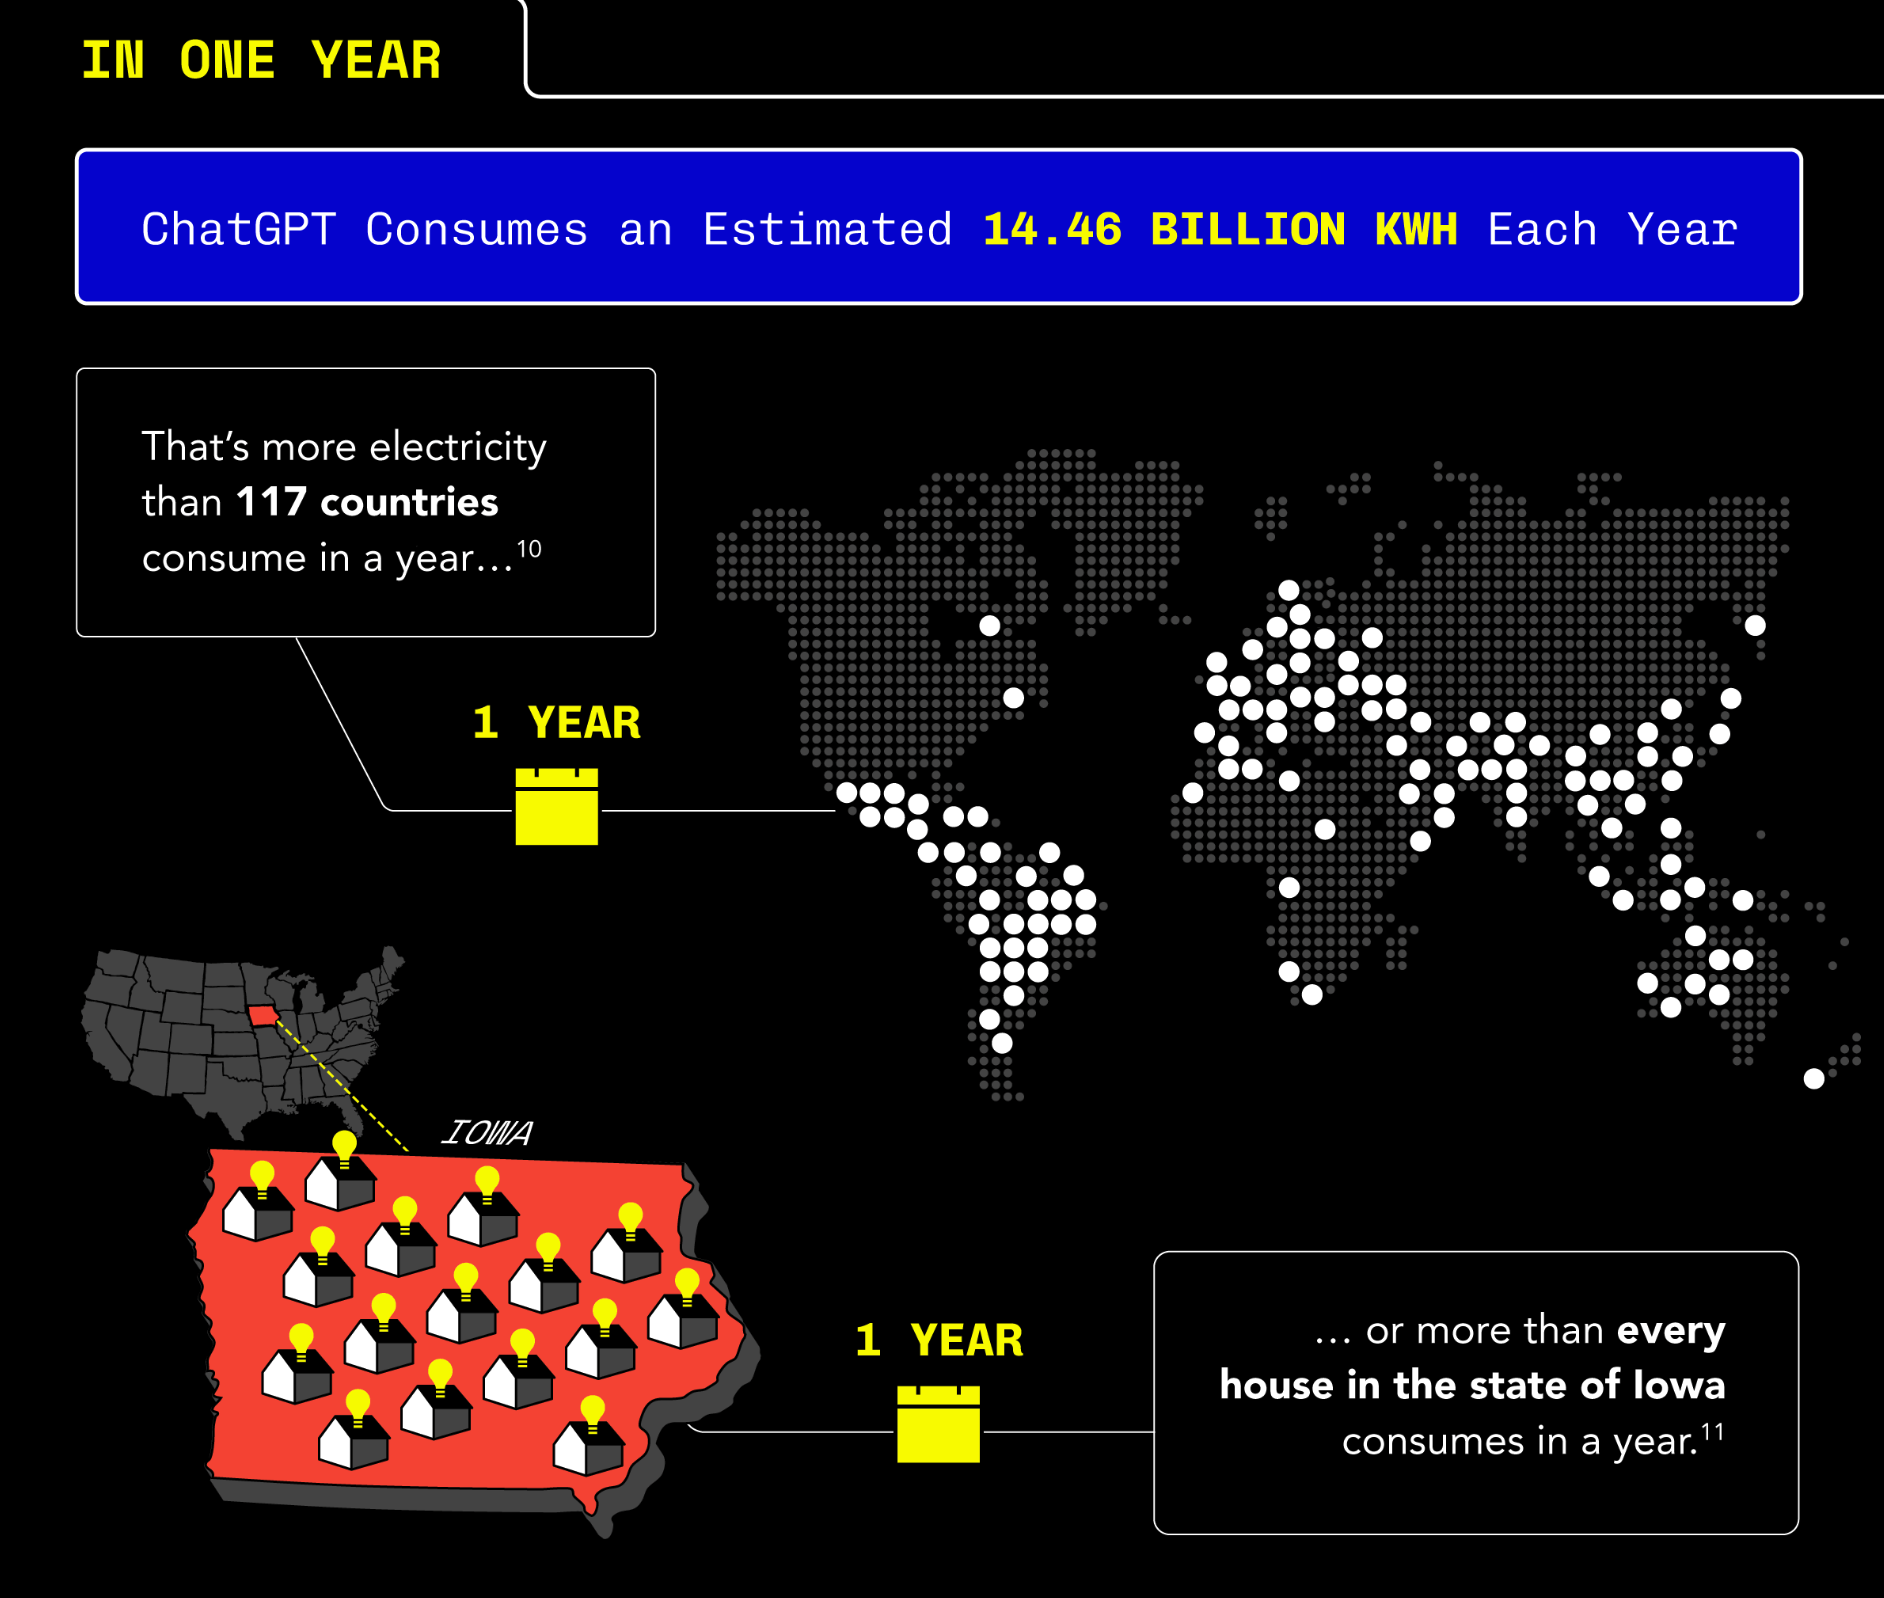
\includegraphics[width=0.7\linewidth]{figures/aitalk1.png}}
Taken from \url{https://www.businessenergyuk.com/knowledge-hub/chatgpt-energy-consumption-visualized/}
\end{frame}

\begin{frame}
\frametitle{And perhaps not environmentally friendly}
\begin{itemize}
\item In Ireland, data centers consume more than 20 percent of the country’s electricity.
\item In Chile, precious aquifers are in danger of depletion.
\item In South Africa, where blackouts have long been routine, data centers are further taxing the national grid.
\item Similar concerns have surfaced in Brazil, Britain, India, Malaysia, the Netherlands, Singapore and Spain and other countries.
\end{itemize}
\end{frame}

\begin{frame}[plain,fragile]
\frametitle{The future is here, sooner than we may think}


% inline figure
\centerline{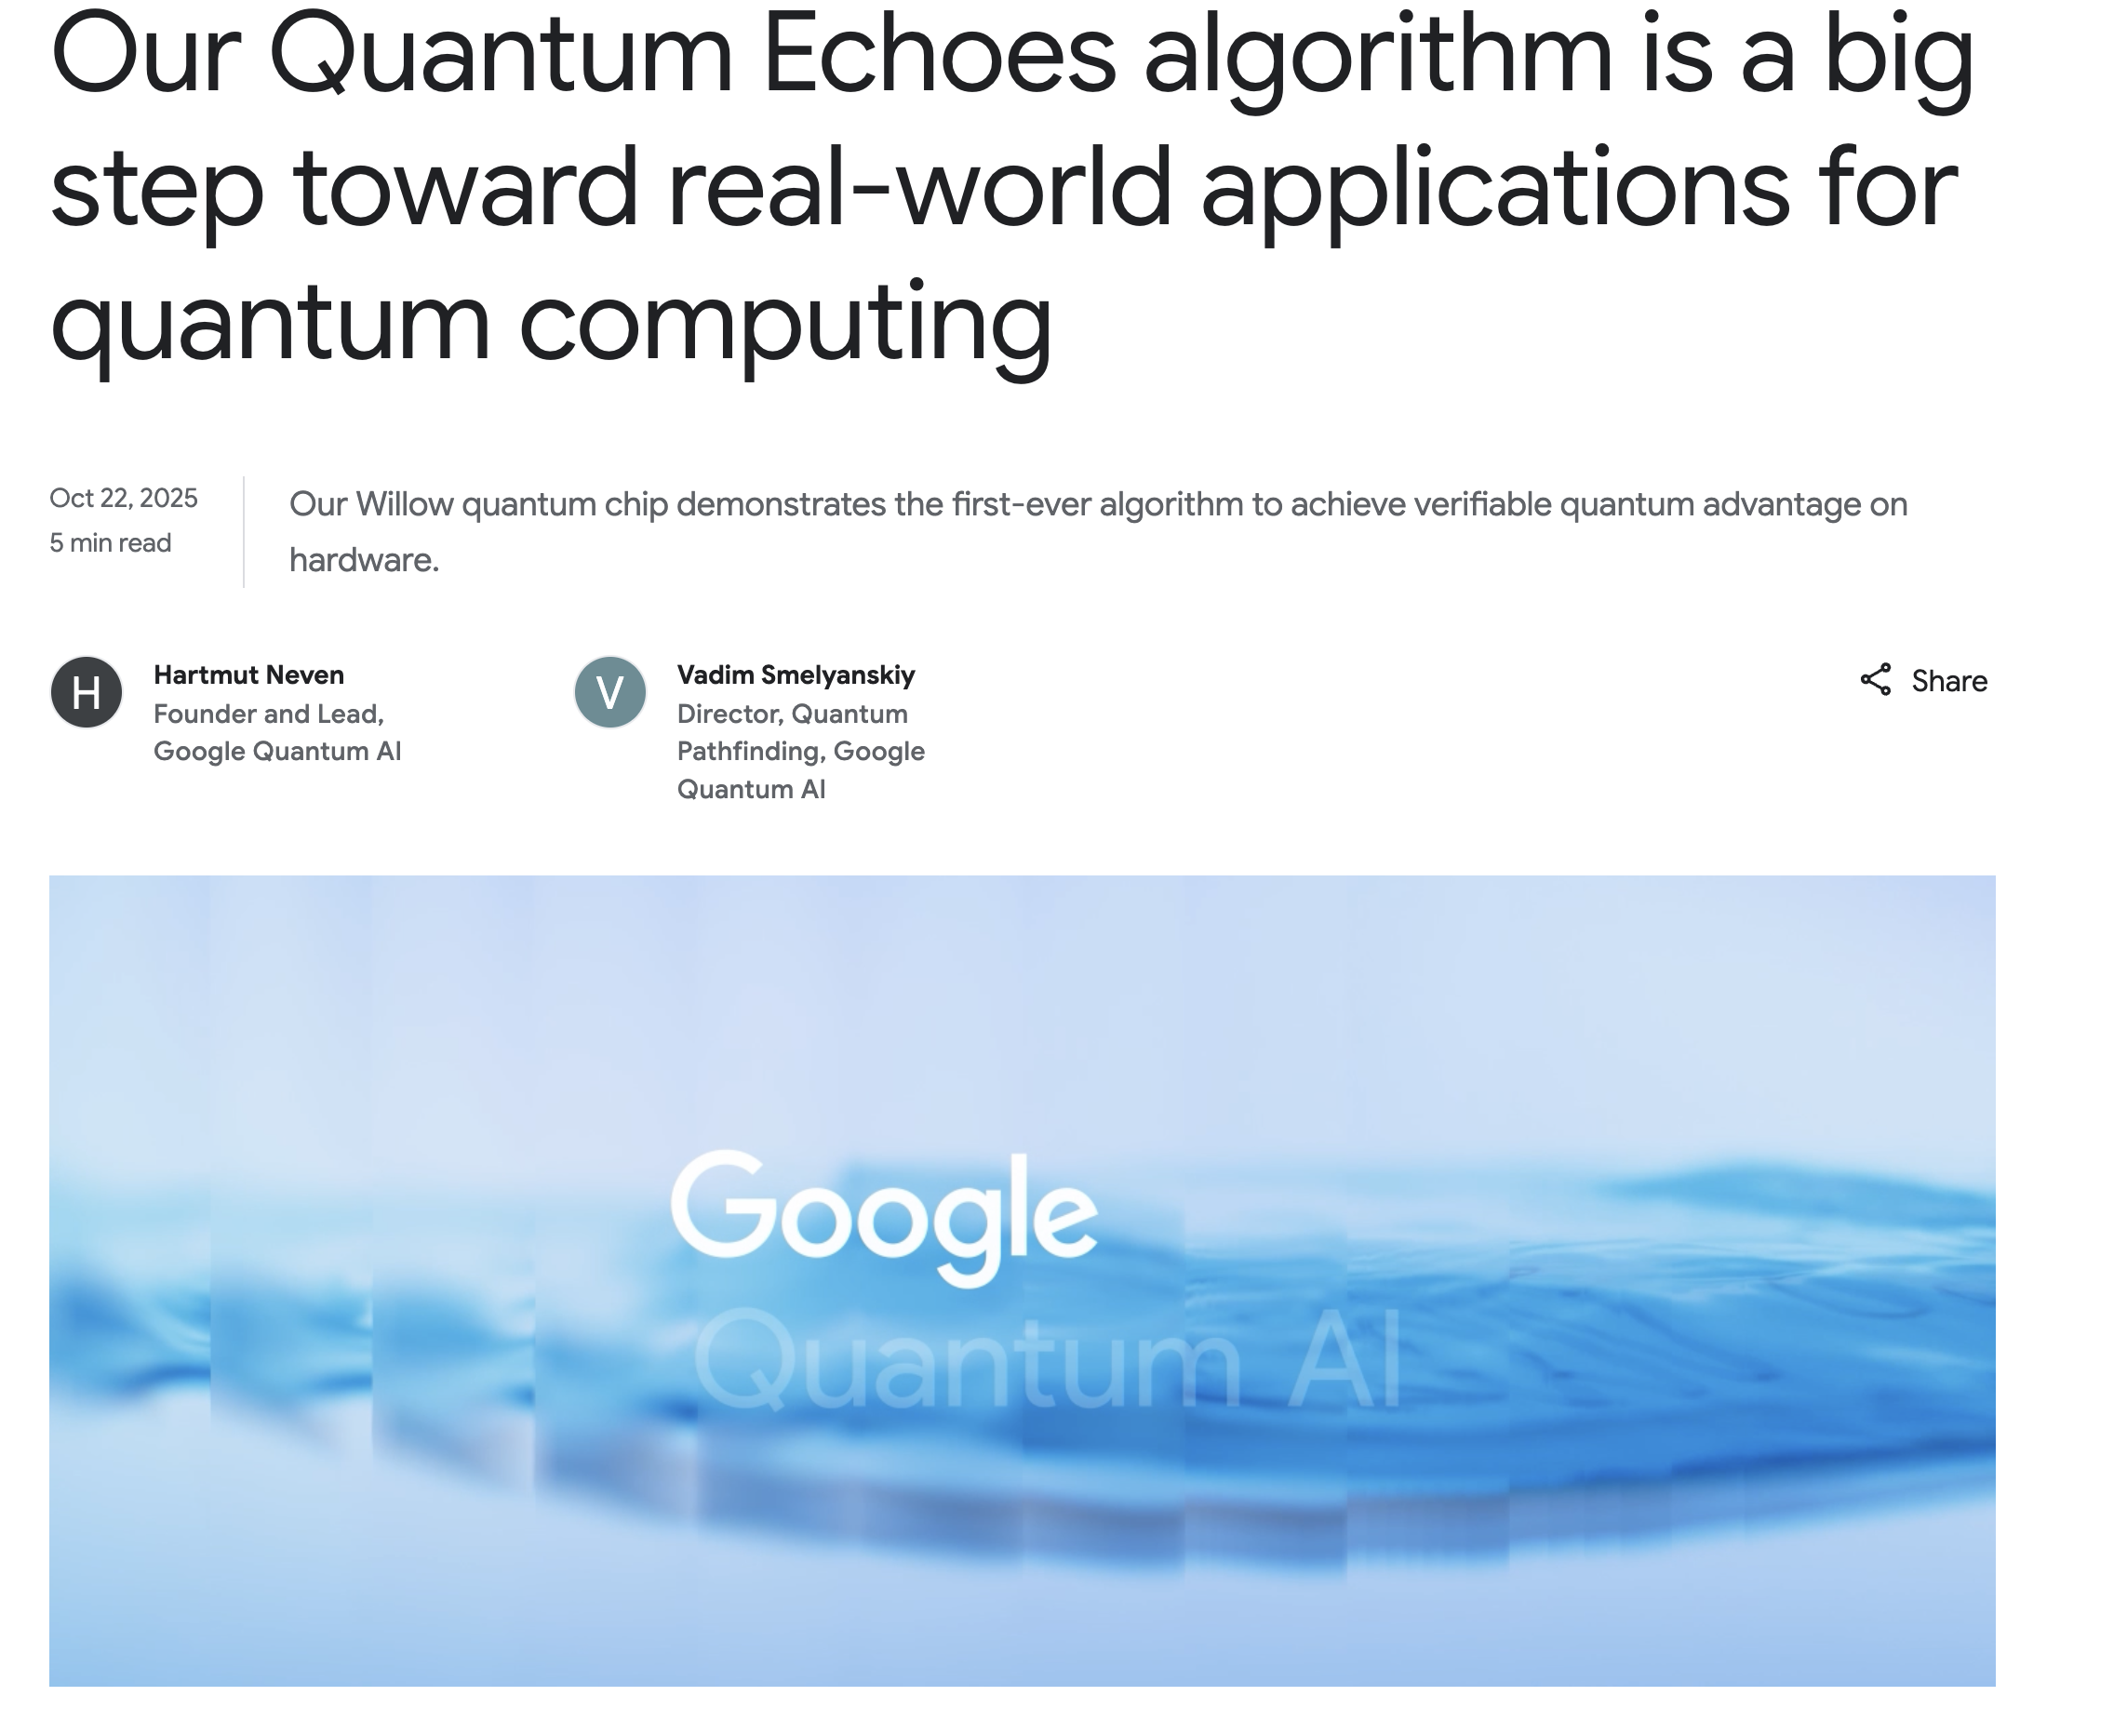
\includegraphics[width=1.05\linewidth]{figures/figuregoogle1.png}}

\end{frame}


\begin{frame}[plain,fragile]
\frametitle{Modern quantum platforms require cooling down to extremely low temperatures}


% inline figure
\centerline{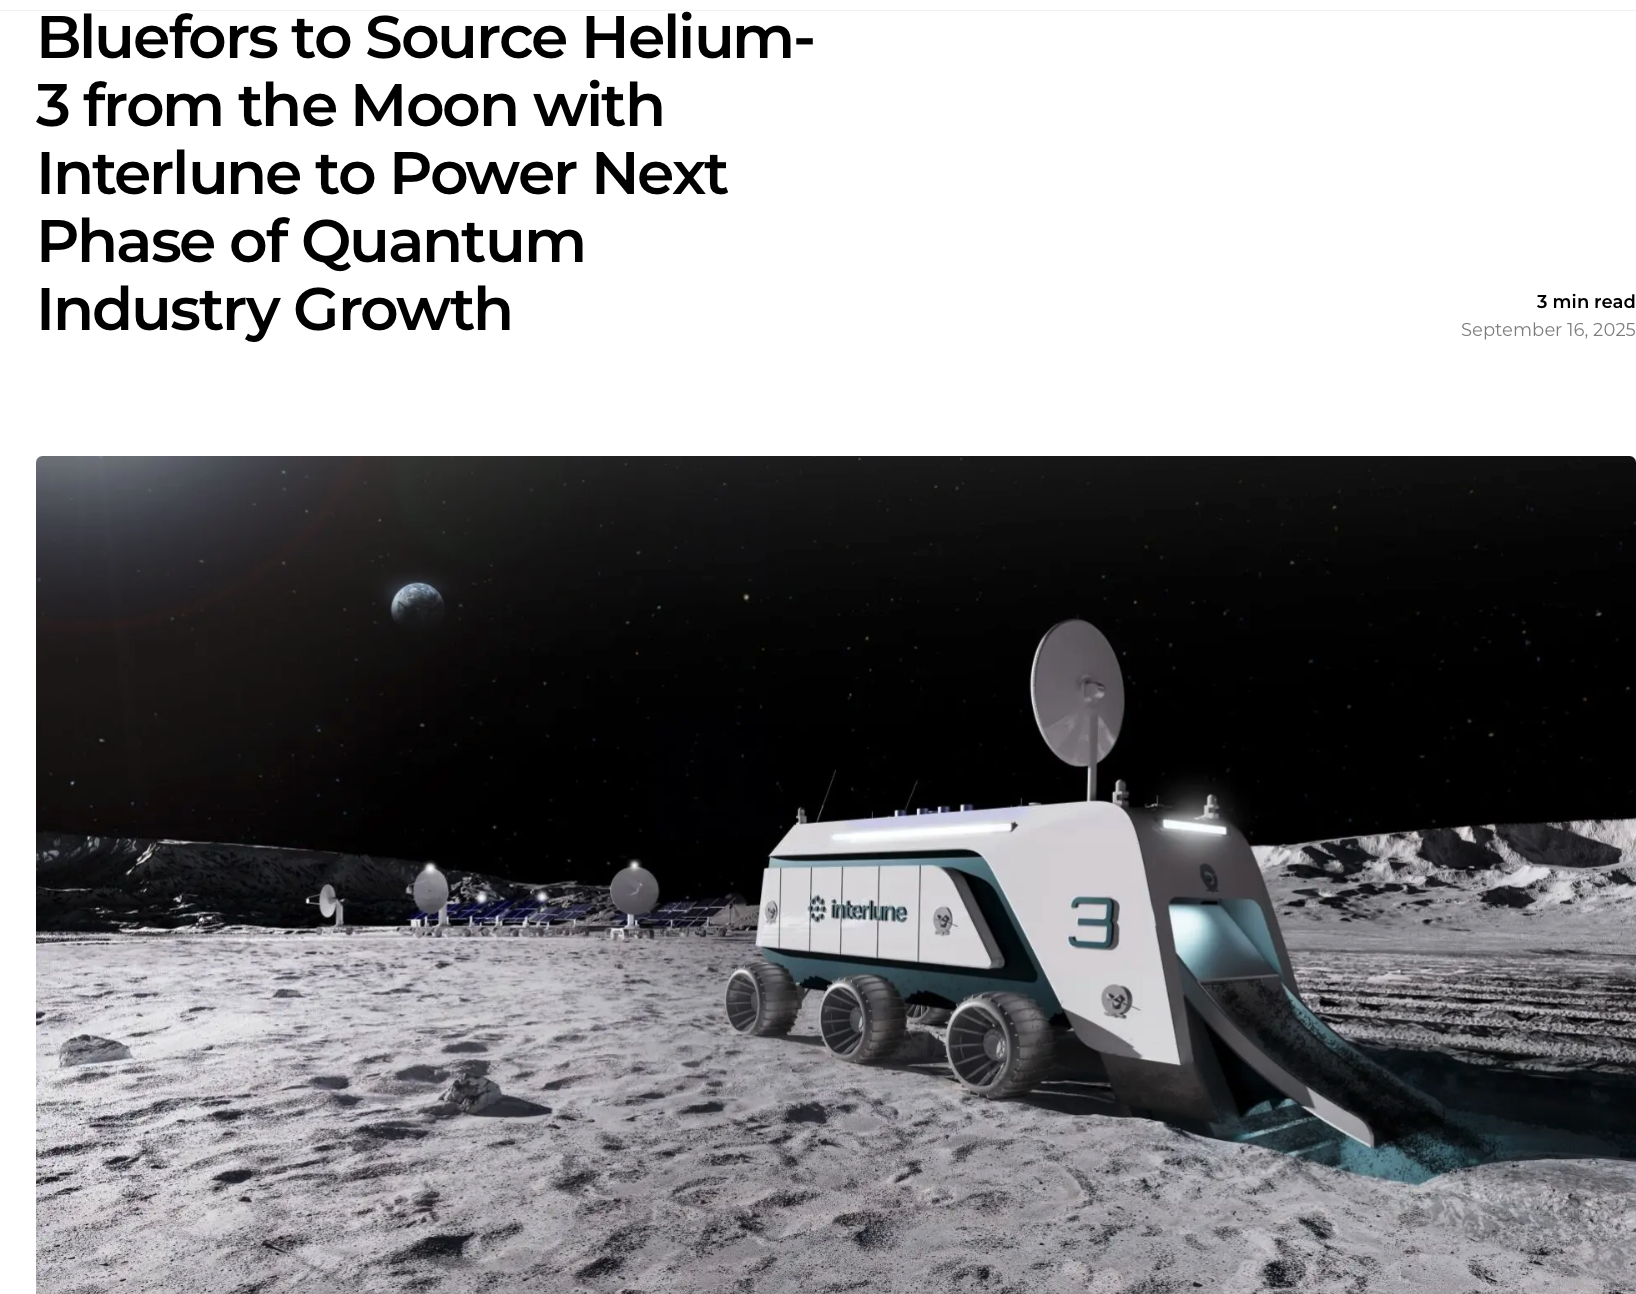
\includegraphics[width=1.05\linewidth]{figures/miningthemoon.png}}

\end{frame}







%==============================================================================
\section{Computational Science and Data Science: The Big Picture}
%==============================================================================

\begin{frame}{A Transformative Moment in Computational Science}

  \begin{columns}[T]
    \begin{column}{0.54\textwidth}
      Two revolutions are unfolding in parallel:
      \medskip
      \begin{itemize}
        \item \textbf{Artificial Intelligence} has transformed data-driven
              modelling, optimization, and prediction
        \medskip
        \item \textbf{Quantum Technologies} promise fundamentally new
              approaches to computing, simulation, sensing, and communication
      \end{itemize}
      \bigskip
      \alert{These two fields are now beginning to influence each other
      in profound ways.}
    \end{column}
    \begin{column}{0.42\textwidth}
      \begin{block}{Three Core Components}
        \begin{enumerate}
          \item High-performance computing (HPC)
          \item Artificial intelligence \& ML
          \item Quantum technologies
        \end{enumerate}
      \end{block}
      \medskip
      \small Together these may form a \textbf{new paradigm} for
      scientific discovery.
    \end{column}
  \end{columns}
\end{frame}

%------------------------------------------------------------------------------
\begin{frame}{The Role of Computational Science Today}

  \begin{itemize}
    \item Computational science is a central pillar of modern research,
          complementing theory \emph{and} experiment
    \medskip
    \item Rapid growth of \textbf{HPC} enables increasingly realistic
          simulations across climate science, neuroscience, materials
          research, and astrophysics
    \medskip
    \item \textbf{AI and ML} have transformed how researchers analyse
          large datasets, discover patterns, and build predictive models
    \medskip
    \item \textbf{Quantum technologies} are now translating fundamental
          quantum-mechanical concepts — superposition, entanglement —
          into practical technologies
  \end{itemize}

  \bigskip
  \begin{center}
    \textcolor{mqblue}{\bfseries
    Quantum computers open new capabilities in simulation,
    optimization, and linear algebra.}
  \end{center}

\end{frame}

%==============================================================================
\section{AI for Quantum Technologies}
%==============================================================================

\begin{frame}{Machine learning meets quantum hardware}

  \begin{columns}[T]
    \begin{column}{0.52\textwidth}
      \textbf{Core challenge:} Quantum devices are delicate systems.
      Small imperfections $\Rightarrow$ decoherence and loss of information.

      \bigskip
      \textbf{Reinforcement learning} has proven particularly powerful:
      \begin{itemize}
        \item Agent interacts with a simulated/experimental quantum system
        \item Learns control protocols that optimize a desired objective
        \item Applications: state preparation, high-fidelity gate implementation
      \end{itemize}
    \end{column}
    \begin{column}{0.44\textwidth}
      \begin{block}{ML Applications to Quantum Hardware}
        \begin{itemize}
          \item Calibration \& characterisation
          \item Error mitigation \& noise reduction
          \item Automated control-sequence discovery
          \item Adaptive quantum experiment design
        \end{itemize}
      \end{block}
      \medskip
      \small Parameter spaces in quantum devices are \textbf{huge}
      — traditional optimization struggles.
    \end{column}
  \end{columns}

\end{frame}

%==============================================================================
\section{Quantum Computing for AI}
%==============================================================================

\begin{frame}{Can quantum hardware accelerate machine learning?}

  \begin{itemize}
    \item Many ML algorithms rely on expensive \textbf{linear algebra}:
          matrix inversion, eigenvalue decomposition, high-dimensional
          optimization
    \medskip
    \item Quantum algorithms have been proposed that may \emph{accelerate}
          certain instances of these tasks: linear systems, sampling,
          optimization
    \medskip
    \item The field of \textbf{quantum machine learning} explores entirely
          new computational models enabled by quantum hardware
  \end{itemize}

  \medskip
  \begin{block}{Hybrid Quantum--Classical Algorithms}
    \begin{itemize}
      \item A classical optimization loop interacts with a quantum
            processor evaluating parameterised quantum circuits
      \item Key framework for \emph{near-term} (NISQ) quantum devices
      \item Practical quantum advantage for ML remains an \textbf{open question}
    \end{itemize}
  \end{block}

\end{frame}

%==============================================================================
\section{A New Paradigm}
%==============================================================================

\begin{frame}{Toward a New Paradigm for Computational Discovery}

  \begin{columns}[T]
    \begin{column}{0.48\textwidth}
      \textbf{Three pillars — distinct but interacting:}
      \medskip
      \begin{enumerate}
        \setlength\itemsep{6pt}
        \item \textcolor{mqblue}{\bfseries High-performance computing}\\
              \small Large-scale simulations, data generation
        \item \textcolor{mqblue}{\bfseries AI and machine learning}\\
              \small Pattern recognition, surrogate modelling, model reduction
        \item \textcolor{mqblue}{\bfseries Quantum technologies}\\
              \small New capabilities for specific hard problems
      \end{enumerate}
    \end{column}
    \begin{column}{0.48\textwidth}
      \textbf{Key implications:}
      \medskip
      \begin{itemize}
        \setlength\itemsep{6pt}
        \item Experiments generate \emph{massive datasets} requiring
              sophisticated analysis
        \item ML can \emph{accelerate} simulations via surrogate models
              and effective physical representations
        \item Quantum technologies may enable simulations of
              \emph{strongly correlated} systems intractable classically
      \end{itemize}
    \end{column}
  \end{columns}

  \bigskip
  \begin{center}
    \textcolor{mqblue}{\bfseries
    Computational science becomes a tightly integrated ecosystem:
    theory, simulation, data analysis, and experiment interact continuously.}
  \end{center}

\end{frame}

%------------------------------------------------------------------------------
\begin{frame}{Conceptual Framework — Three Pillars of Future Discovery}
%  \framesubtitle{Figure placeholder}

  \begin{center}
    \begin{tikzpicture}[scale=0.92]
      % Placeholder rectangle
      \draw[mqblue, line width=1.5pt, dashed, rounded corners=4pt]
        (0,0) rectangle (12,5.8);
      \node[mqgray, font=\large\bfseries] at (6,3.5)
        {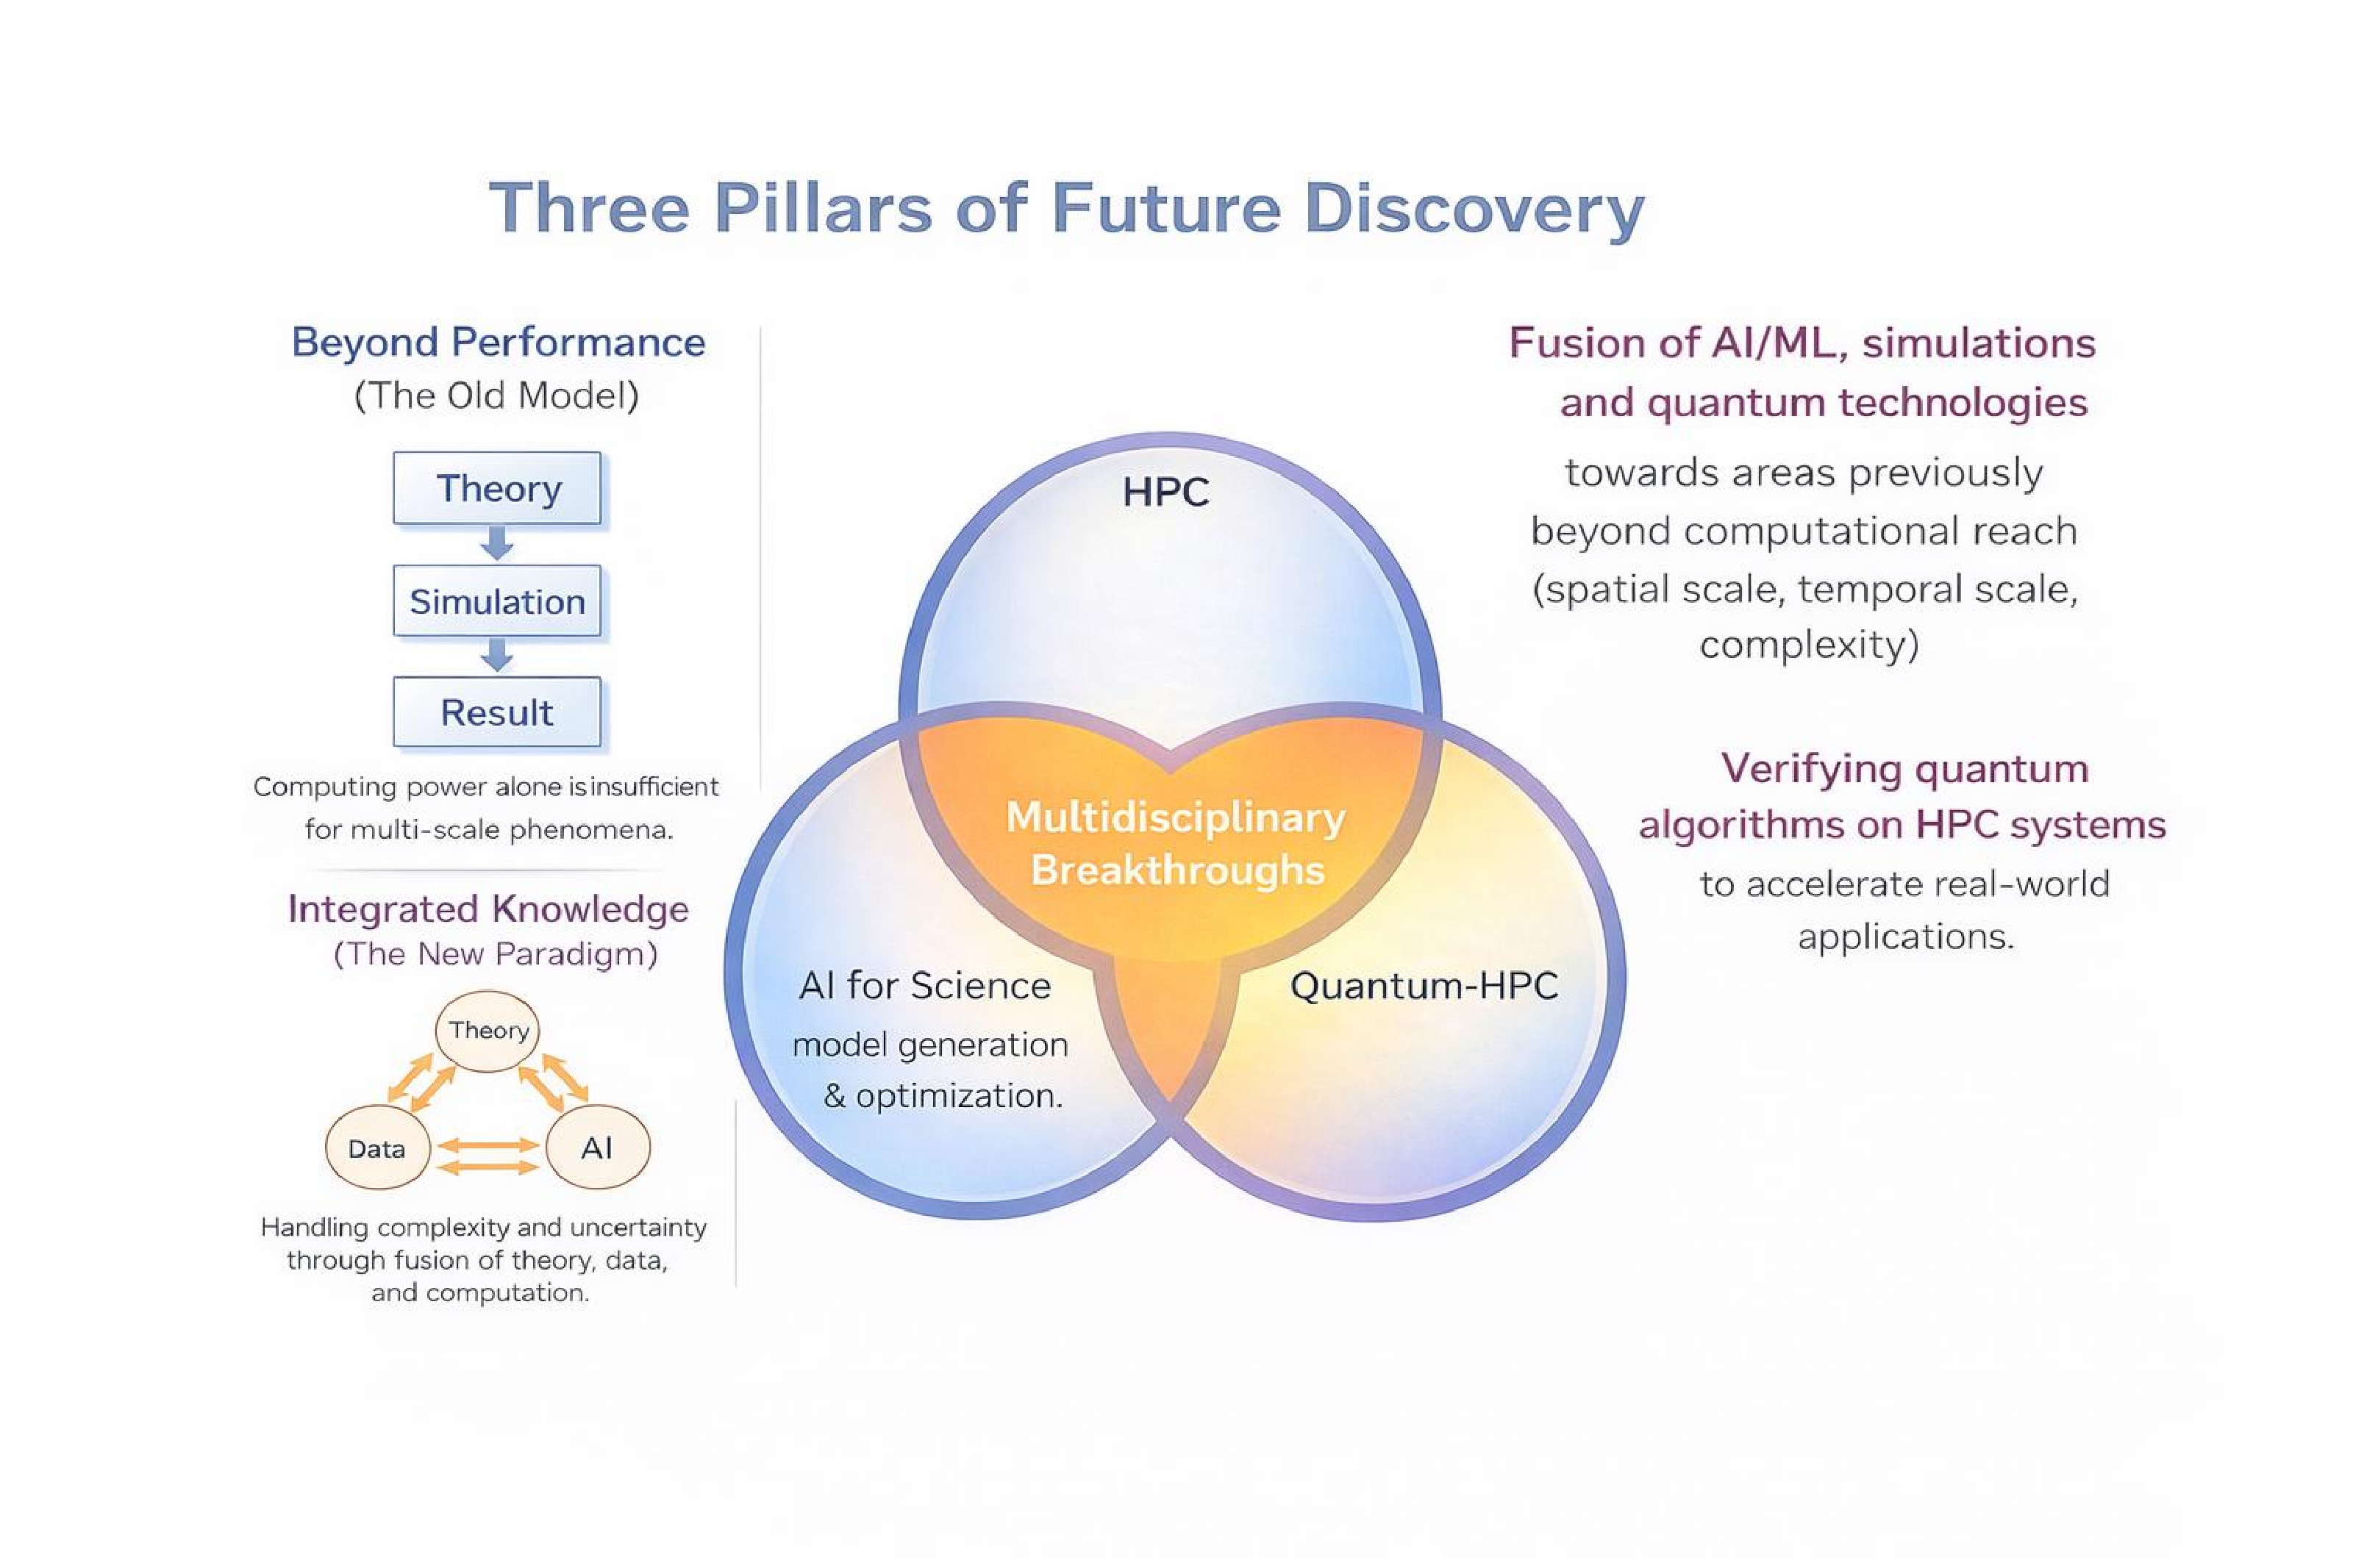
\includegraphics[width=0.9\linewidth]{Futurevision.pdf}};
    \end{tikzpicture}
  \end{center}

\end{frame}



\begin{frame}[plain,fragile]
\frametitle{Quantum technology and machine learning/AI}


% inline figure
\centerline{\includegraphics[width=1.05\linewidth]{figureintro.pdf}}

\end{frame}

%-----------------------------------------------------------
\section{Quantum computing in brief}
\begin{frame}{What is Quantum Computing?}
Quantum computing leverages principles of quantum mechanics to perform computations beyond classical capabilities.

\vspace{10pt}
\textbf{Key Concepts:}
\begin{itemize}
\item \textbf{Superposition:} Qubits can exist in a combination of states.
\item \textbf{Entanglement:} Correlation between qubits regardless of distance.
\item \textbf{Quantum Interference:} Probability amplitudes interfere to solve problems.
\end{itemize}
\end{frame}
%-----------------------------------------------------------

\begin{frame}{What is Quantum Machine Learning?}
\textbf{Quantum Machine Learning (QML)} integrates quantum computing with machine learning algorithms to exploit quantum advantages.

\vspace{10pt}
\textbf{Motivation:}
\begin{itemize}
    \item High-dimensional Hilbert spaces for better feature representation.
    \item Quantum parallelism for faster computation.
    \item Quantum entanglement for richer data encoding.
\end{itemize}


\end{frame}

\begin{frame}{Quantum Speedups in ML}
\textbf{Why Quantum?}
\begin{itemize}
    \item \textbf{Quantum Parallelism:} Process multiple states simultaneously.
    \item \textbf{Quantum Entanglement:} Correlated states for richer information.
    \item \textbf{Quantum Interference:} Constructive and destructive interference to enhance solutions.
\end{itemize}

\textbf{Advantage:}
Speedups in high-dimensional optimization and linear algebra problems.
\end{frame}

%-----------------------------------------------------------

\begin{frame}{Challenges and Limitations}
\textbf{Quantum Hardware Limitations:}
\begin{itemize}
    \item Noisy Intermediate-Scale Quantum (NISQ) devices.
    \item Decoherence and limited qubit coherence times.
\end{itemize}

\textbf{2. Data Encoding:}
\begin{itemize}
    \item Efficient embedding of classical data into quantum states.
\end{itemize}

\textbf{3. Scalability:}
\begin{itemize}
    \item Difficult to scale circuits to large datasets.
\end{itemize}
\end{frame}



\begin{frame}[plain,fragile]
\frametitle{Quantum Metrology}

\textbf{Quantum Metrology:}
\begin{itemize}
    \item Uses entangled states for ultra-precise measurements.
    \item Overcomes the classical shot-noise limit.
\end{itemize}

\textbf{Heisenberg Limit:}
\[
\Delta \theta \ge \frac{1}{N},
\]

where \( N \) is the number of entangled particles.  

\begin{block}{Advantage:}
\begin{itemize}
\item Quantum entanglement improves sensitivity beyond classical limits.
\end{itemize}
\end{block}
\end{frame}

\begin{frame}{Challenges of Quantum Entanglement}
\textbf{Decoherence:}
\begin{itemize}
    \item Entangled states are fragile.
    \item Interaction with the environment collapses the wavefunction.
\end{itemize}

\textbf{Scalability:}
\begin{itemize}
    \item Difficult to entangle large numbers of qubits.
    \item Error correction requires complex protocols.
\end{itemize}

\textbf{Measurement Problem:}
\begin{itemize}
    \item Measurement destroys entanglement.
    \item Trade-off between information gain and entanglement preservation.
\end{itemize}
\end{frame}


%==============================================================================
\section{Case Studies}
%==============================================================================

\begin{frame}{Case Studies — Overview}

  \begin{columns}[T]
    \begin{column}{0.48\textwidth}
      \begin{block}{Quantum Control}
        RL and neural-network optimization discover control strategies
        that \emph{outperform} traditional approaches for quantum
        computers and sensors
      \end{block}
      \medskip
      \begin{block}{Quantum Simulation of Many-Body Systems}
        Classical approaches face \emph{exponential} complexity for
        strongly correlated systems; hybrid quantum-classical methods
        may provide new tools
      \end{block}
      \medskip
      \begin{block}{AI-Assisted Hardware Development}
        ML analyses experimental data, identifies noise sources, and
        optimizes device architectures — accelerating the path to
        fault-tolerant quantum computers
      \end{block}
    \end{column}
    \begin{column}{0.48\textwidth}
      \begin{block}{Quantum ML for Finance}
        \begin{itemize}
          \item Portfolio optimization via QAOA / quantum annealing
          \item Quantum kernel methods for financial time series
          \item Quantum generative models for risk analysis and
                Monte-Carlo-style simulations
        \end{itemize}
      \end{block}
      \medskip
      \begin{block}{Applications to Neuroscience}
        \begin{itemize}
          \item QML for high-dimensional neural data representation
          \item Quantum simulation of spin-model-like neural dynamics
        \end{itemize}
      \end{block}
    \end{column}
  \end{columns}

\end{frame}

%------------------------------------------------------------------------------
\begin{frame}{Spotlight: Quantum Control with Reinforcement Learning}

  \begin{columns}[T]
    \begin{column}{0.52\textwidth}
      \textbf{Why is control hard?}
      \begin{itemize}
        \item Parameter spaces of quantum devices are extremely large
        \item Traditional optimization methods scale poorly
        \item Noise and decoherence degrade any imperfect protocol
      \end{itemize}
      \bigskip
      \textbf{What RL offers:}
      \begin{itemize}
        \item Model-free exploration of huge control landscapes
        \item Discovers non-intuitive protocols
        \item Adapts online to hardware drift
      \end{itemize}
    \end{column}
    \begin{column}{0.44\textwidth}
      \begin{block}{Key References}
        \footnotesize
        \begin{itemize}
          \item Bukov \& Marquardt,
                \emph{RL for Quantum Technology},
                arXiv:2601.18953 (2026)
          \item Belliardo et al.,
                \emph{Model-aware RL for Bayesian quantum metrology},
                Quantum \textbf{8}, 1555 (2024)
        \end{itemize}
      \end{block}
      \medskip
      \small
      \textcolor{mqblue}{Result:} RL agents have demonstrated gate
      fidelities competitive with hand-tuned protocols on real hardware.
    \end{column}
  \end{columns}

\end{frame}

%------------------------------------------------------------------------------
\begin{frame}{Spotlight: Quantum ML for Finance and Neuroscience}

  \begin{columns}[T]
    \begin{column}{0.48\textwidth}
      \textbf{Finance}
      \begin{itemize}
        \item Large datasets, stochastic dynamics,
              high-dimensional optimization
        \item \textbf{QAOA} / quantum annealing for combinatorial
              portfolio optimization
        \item \textbf{Quantum kernel methods} — data encoded in
              quantum states; similarity evaluated in Hilbert space
        \item \textbf{Quantum generative models} — variational circuits
              or quantum Boltzmann machines for risk analysis
      \end{itemize}
    \end{column}
    \begin{column}{0.48\textwidth}
      \textbf{Neuroscience}
      \begin{itemize}
        \item Brain: billions of interacting neurons, highly complex
              dynamical system
        \item ML already central for analysing neural recordings
        \item \textbf{QML} may represent high-dimensional neural data
              or model complex probability distributions
        \item Models of collective neural behaviour resemble
              \textbf{spin systems} from statistical physics
              $\Rightarrow$ methods from quantum many-body physics
              may offer new insights
      \end{itemize}
    \end{column}
  \end{columns}

\end{frame}

%==============================================================================
\section{Future Strategies}
%==============================================================================

\begin{frame}{Future Strategies and Requirements}

  \begin{columns}[T]
    \begin{column}{0.32\textwidth}
      \begin{block}{\centering Interdisciplinary\\Collaboration}
        \centering\medskip
        Physics $\;\cdot\;$ Computer science $\;\cdot\;$
        Mathematics $\;\cdot\;$ Engineering
        \medskip

        \small Key challenges lie \emph{at the intersection}
        of these fields
      \end{block}
    \end{column}
    \begin{column}{0.32\textwidth}
      \begin{block}{\centering Education \&\\Training}
        \centering\medskip
        Future researchers need expertise in:
        \medskip

        \small Physics $\;\cdot\;$ Numerical methods $\;\cdot\;$
        Machine learning $\;\cdot\;$ Quantum information science
      \end{block}
    \end{column}
    \begin{column}{0.32\textwidth}
      \begin{block}{\centering Research\\Infrastructure}
        \centering\medskip
        Integrated platforms combining:
        \medskip

        \small HPC resources $\;\cdot\;$ Experimental quantum platforms $\;\cdot\;$
        ML-driven analysis environments
      \end{block}
    \end{column}
  \end{columns}

  \bigskip
  \begin{center}
    \textcolor{mqblue}{\bfseries
    Realising this potential requires coordinated efforts across
    multiple disciplines — no single community can do it alone.}
  \end{center}

\end{frame}


%==============================================================================
\section{Reinforcement Learning and Quantum Control}
%==============================================================================


%================================================
\begin{frame}{Reinforcement Learning and Quantum Control: Motivation}
Many problems in physics can be phrased as optimization problems:
\begin{itemize}
\item variational calculations,
\item control of dynamical systems,
\item adaptive measurements,
\item maximizing sensitivity in quantum sensors.
\end{itemize}

However, in many realistic settings:
\begin{itemize}
\item the objective is not known analytically,
\item gradients are unavailable or noisy,
\item decisions must be taken sequentially,
\item present choices affect future opportunities.
\end{itemize}

Reinforcement learning (RL) addresses precisely this type of problem.
\end{frame}



\begin{frame}{Quantum Control}
\centerline{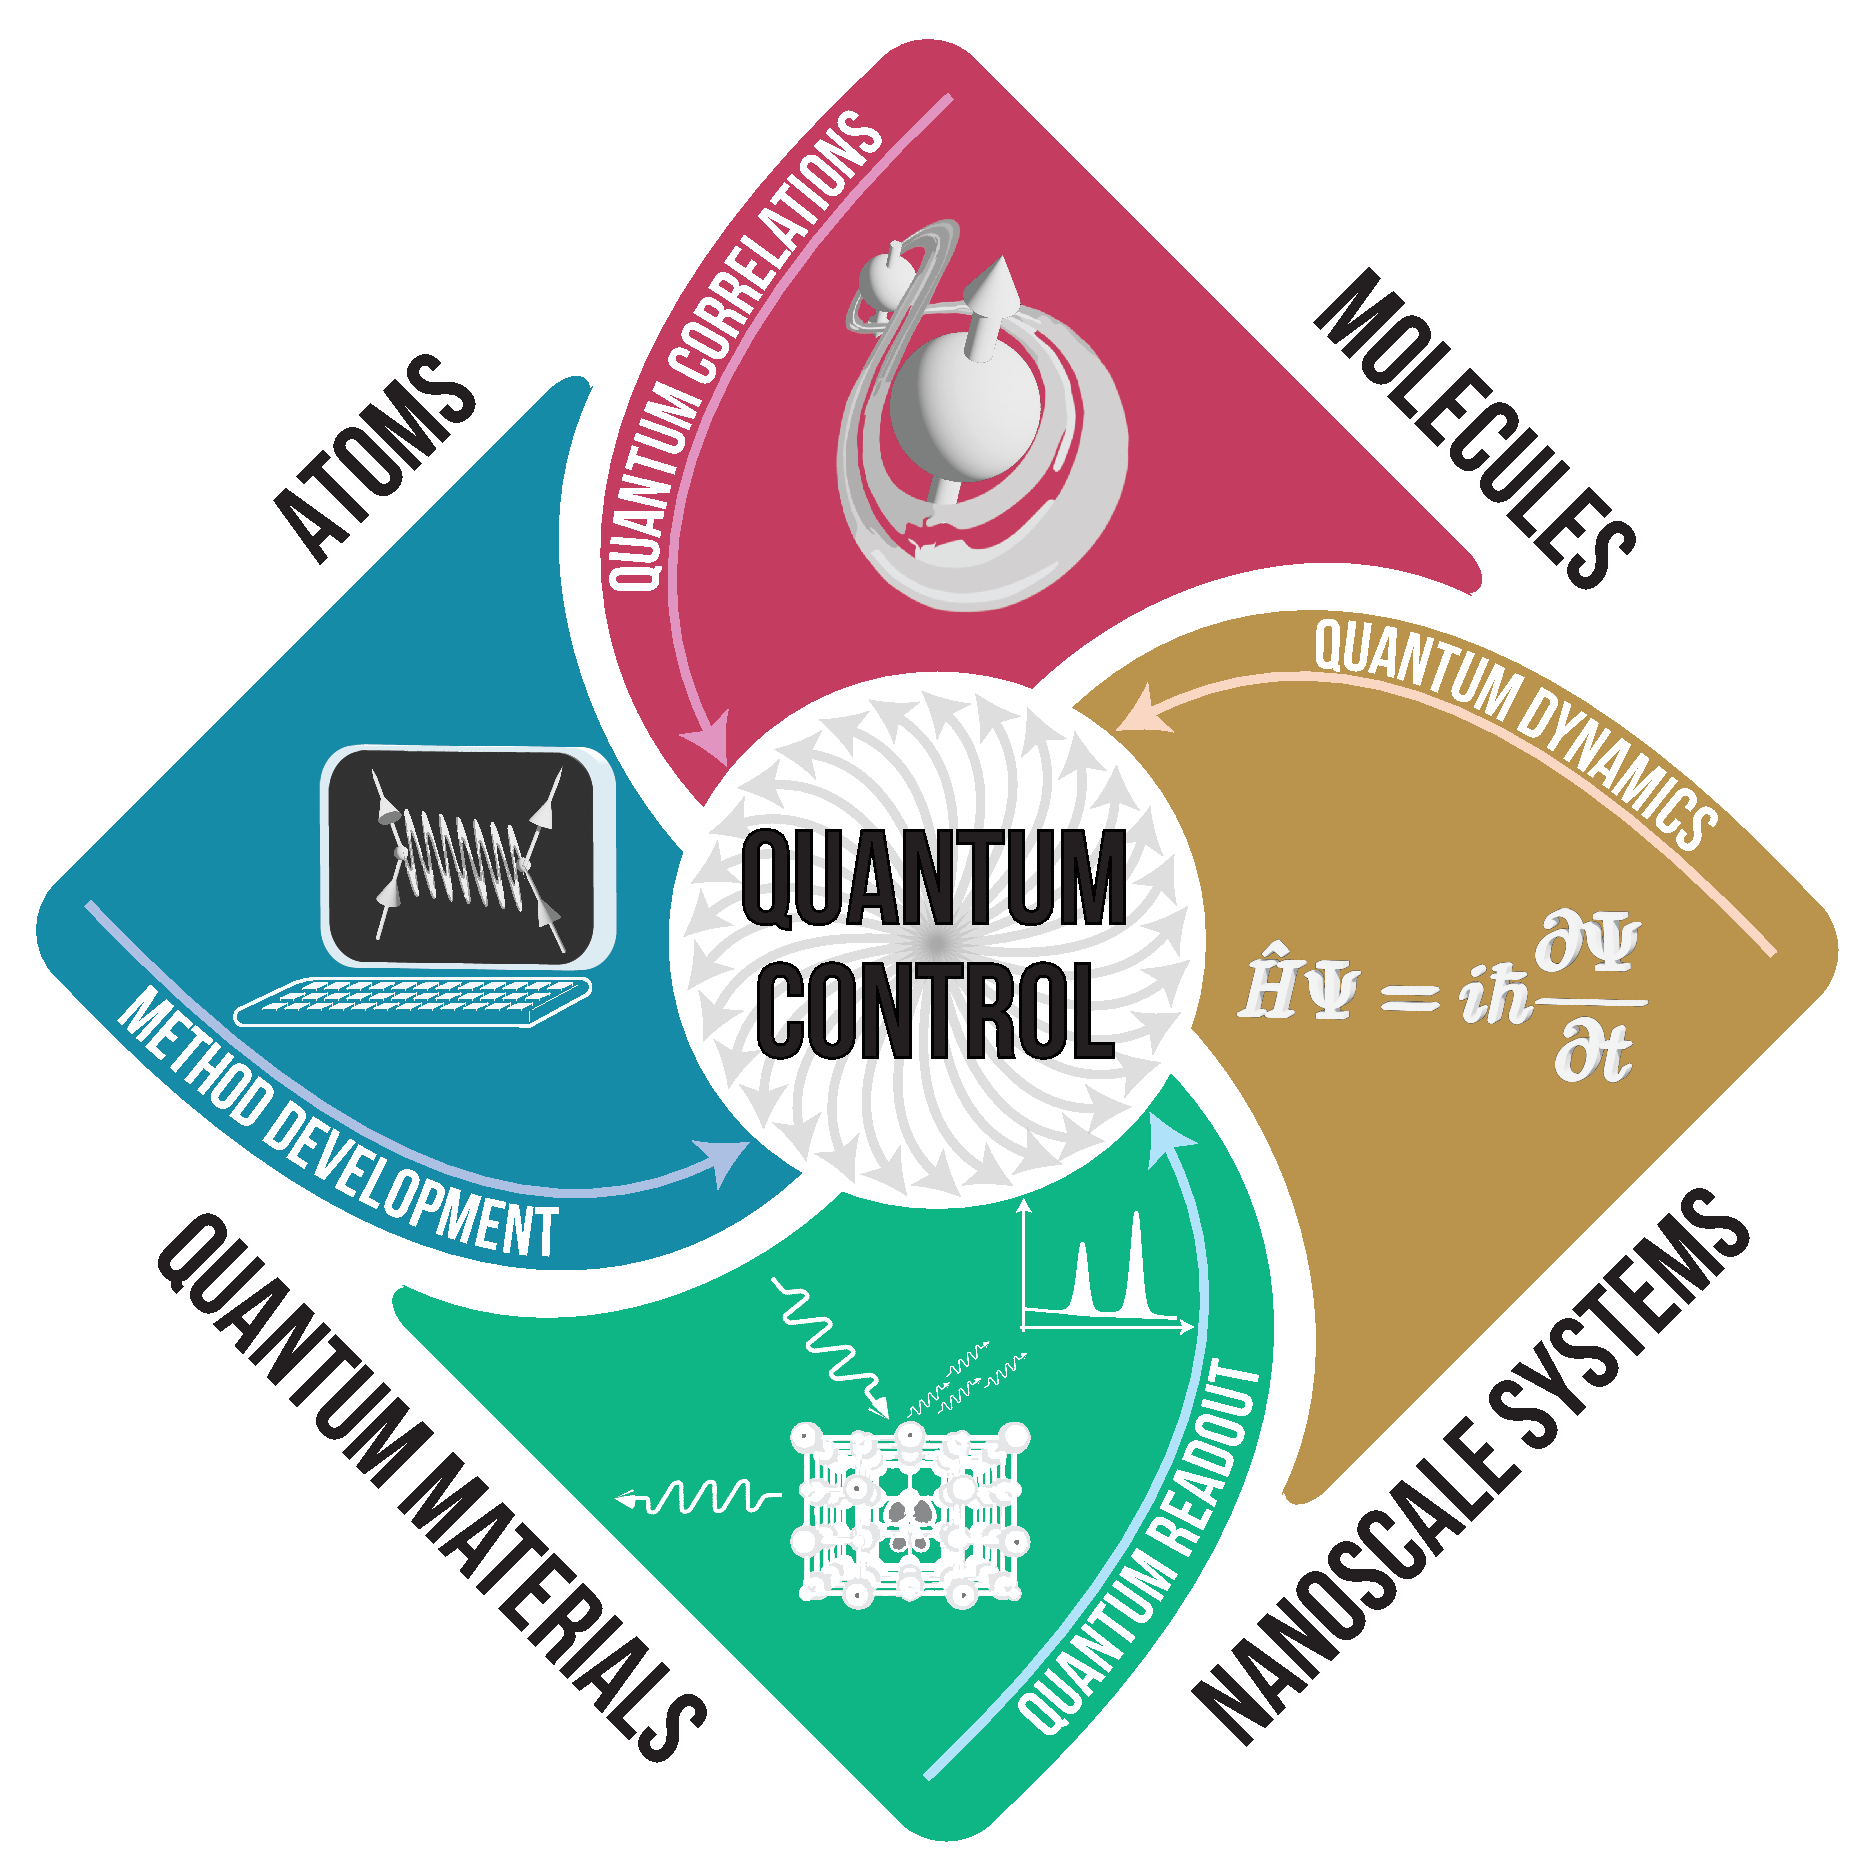
\includegraphics[width=0.5\linewidth]{quantumcontrol.pdf}}
\end{frame}




\begin{frame}{What is Reinforcement Learning? In plain words}
\begin{block}{}  

The RL framework consists of an {\bf agent} that learns how to solve a
task by interacting with a physical system, called the
environment. The agent can select {\bf actions} that modify the {\bf
  state} of the environment, as a consequence a {\bf reward} is given
to the agent, and the process repeats in a positive feedback loop. The
objective is to maximise the sum of expected rewards andf thereby
accomplish the task. The agent learns a {\bf strategy} that can be
meployed under similar yet different circumstances. The so-called {\bf
  policy} os the rule for choosing actions.

\end{block}
\end{frame}


\begin{frame}{My more narrow motivation (another talk perhaps)}
\begin{itemize}
  \item Quantum sensors permit fine-grained control over probe evolution and measurement settings.
  \item The central design problem is sequential: which control should be applied \emph{next}, given what has already been learned?
  \item For realistic platforms, the estimation stack contains many non-smooth components: sampling of measurement outcomes, particle-filter resampling, and optional weak-measurement backaction.
  \item The article by Belliardo {\em et al.} (UniPI, SNS)  proposes a \alert{model-aware RL} framework that treats experimental design as a trainable control problem while retaining a faithful physical model.
\end{itemize}
\end{frame}


%================================================
\begin{frame}{What is Reinforcement Learning?}
  An agent interacts with an environment over discrete time steps:
  \[
  s_0,a_0,r_1,s_1,a_1,r_2,\dots
  \]

  Core ingredients:
  \begin{itemize}
  \item \textbf{State} $s_t$: information available at time $t$,
  \item \textbf{Action} $a_t$: decision taken by the agent,
  \item \textbf{Reward} $r_{t+1}$: feedback from the environment,
  \item \textbf{Policy} $\pi(a|s)$: rule for choosing actions.
  \end{itemize}

  Goal:
  \[
  \max_\pi \; \mathbb{E}_\pi\!\left[\sum_{t=0}^{\infty}\gamma^t r_{t+1}\right]
  \]
  where $0\le \gamma <1$ is a discount factor.
\end{frame}

%================================================
\begin{frame}{Sequential Decision Making}
  In ordinary optimization we choose parameters once.

  In reinforcement learning we choose a \emph{sequence} of actions:
  \[
  a_0,a_1,a_2,\dots
  \]

  This matters because:
  \begin{itemize}
  \item actions change the future state,
  \item the future state changes which actions are useful later,
  \item rewards may be delayed.
  \end{itemize}

  Thus RL is best viewed as \textbf{optimization over trajectories or strategies}.
\end{frame}



\begin{frame}{Model-aware RL}
\begin{block}{Core idea}
Use a differentiable simulation of the experiment, Bayesian inference by particle filtering, and policy optimization to learn adaptive or non-adaptive control laws for quantum metrology.
\end{block}
\begin{itemize}
  \item \textbf{Bayesian mode:} optimize the final estimation error after a complete measurement sequence.
  \item \textbf{Frequentist mode:} optimize the Cramer-Rao bound through the Fisher information matrix.
  \item \textbf{Model-aware:} gradients are propagated through a known sensor model rather than inferred only from trial-and-error interaction.
\end{itemize}
\end{frame}

\begin{frame}{The measurement loop as a control architecture}
\begin{enumerate}
  \item From the current posterior summary, the agent outputs the next control $x_{t+1}$.
  \item The probe evolves and is measured, producing a stochastic outcome $y_{t+1}$.
  \item The Bayesian posterior is updated and fed back to the agent.
\end{enumerate}
\vspace{0.5em}
Adaptive policies are written as
\[
  x_{t+1}=F_{\lambda}\!\big(P(\theta\mid x_t,y_t);\, y_t;\, R_t;\, t\big),
\]
while non-adaptive strategies suppress dependence on the posterior and outcomes:
\[
  x_{t+1}=F_{\lambda}(R_t,t).
\]
\begin{itemize}
  \item $\lambda$: trainable parameters of the policy (typically a neural network).
  \item $R_t$: resources consumed up to step $t$ (time, photons, signal amplitude, \ldots).
\end{itemize}
\end{frame}


%================================================
\begin{frame}{Model-Free vs Model-Aware Reinforcement Learning}
  Two broad philosophies:

  \textbf{Model-free RL}
  \begin{itemize}
  \item learn directly from transitions,
  \item no explicit model of $P(s'|s,a)$ is used,
  \item examples: Q-learning, REINFORCE.
  \end{itemize}

  \textbf{Model-aware (or model-based) RL}
  \begin{itemize}
  \item use or learn a model of the dynamics,
  \item plan using that model,
  \item combine prediction and control.
  \end{itemize}

  In physics, model-aware RL is often especially attractive because we frequently know at least part of the dynamics.
\end{frame}

%================================================
\begin{frame}{What is Model-Aware Reinforcement Learning?}
  In model-aware RL we assume access to:
  \begin{itemize}
  \item known transition probabilities $P(s'|s,a)$, or
  \item an approximate learned model $\hat P_\phi(s'|s,a)$.
  \end{itemize}

  Then we can:
  \begin{itemize}
  \item simulate hypothetical futures,
  \item estimate returns before acting,
  \item plan over multiple time steps,
  \item use differentiable dynamics when available.
  \end{itemize}

  This is close in spirit to standard computational physics:
  \[
  \text{equations of motion} \;\Rightarrow\; \text{simulation} \;\Rightarrow\; \text{optimization}.
  \]
\end{frame}

%================================================
\begin{frame}{Benefits of Model-Aware RL}
  Advantages:
  \begin{itemize}
  \item better sample efficiency,
  \item ability to plan ahead,
  \item easier incorporation of prior physical knowledge,
  \item natural interface with control theory.
  \end{itemize}

  Disadvantages:
  \begin{itemize}
  \item model bias if the model is wrong,
  \item errors may accumulate during planning,
  \item learning an accurate model may be difficult.
  \end{itemize}

  Thus model-aware RL is especially useful when the dynamics are fairly well understood, but the control task remains hard.
\end{frame}

%================================================
\begin{frame}{Model-Aware RL and Physics}
  In many physics applications we know the dynamics:
  \[
  \dot x = f(x,u)
  \]
  or in quantum mechanics
  \[
  i\hbar \frac{d}{dt}\vert \psi(t)\rangle =H(u(t))\vert \psi(t)\rangle.
  \]

  Then the environment is not a black box:
  \begin{itemize}
  \item we can simulate trajectories,
  \item estimate gradients,
  \item evaluate candidate policies offline.
  \end{itemize}

  Model-aware RL thus sits naturally between:
  \begin{itemize}
  \item optimal control,
  \item stochastic optimization,
  \item machine learning.
  \end{itemize}
\end{frame}


%================================================
\begin{frame}{Transition to Quantum Systems}
  Quantum control problems are naturally sequential:
  \begin{itemize}
  \item apply pulse,
  \item observe state evolution,
  \item choose next pulse,
  \item optimize final performance.
  \end{itemize}

  This makes RL conceptually attractive.
At the same time, quantum dynamics are often known from the Schr\"odinger equation, which makes model-aware RL particularly relevant.
\end{frame}

%================================================
\begin{frame}{Quantum Control}
  Quantum dynamics:
  \[
  i\hbar \frac{d}{dt}\vert \psi(t)\rangle = H(t)\vert \psi(t)\rangle.
  \]

  Controlled Hamiltonian:
  \[
  H(t)=H_0+\sum_k u_k(t)H_k
  \]

  Typical goals:
  \begin{itemize}
  \item state preparation,
  \item gate synthesis,
  \item suppression of decoherence,
  \item enhancement of sensor performance.
  \end{itemize}
\end{frame}


%================================================
\begin{frame}{RL Formulation for Quantum Control}
  Mapping:
  \begin{itemize}
  \item \textbf{State}: wavefunction, density matrix, or measurement record,
  \item \textbf{Action}: control amplitude or pulse choice,
  \item \textbf{Reward}: fidelity, energy, Fisher information, robustness.
  \end{itemize}

  Examples of terminal rewards:
  \[
  R = |\langle \psi_{\mathrm{target}}|\psi(T)\rangle|^2
  \]
  or
  \[
  R = F_Q(T)
  \]
  for a quantum sensing task.
\end{frame}

%================================================
\begin{frame}{Quantum Sensors and Fisher Information}
  A quantum sensor estimates a parameter $\theta$.

  Precision is bounded by the quantum Cram\'er--Rao bound:
  \[
  \Delta \theta \ge \frac{1}{\sqrt{\nu F_Q}}
  \]
  where:
  \begin{itemize}
  \item $F_Q$ is the quantum Fisher information,
  \item $\nu$ is the number of repetitions.
  \end{itemize}

  Thus maximizing $F_Q$ is a natural control objective for reinforcement learning.
\end{frame}

\begin{frame}{Worked Quantum Example: Two-Level Sensor}
  Consider a qubit sensing a magnetic field $B$:
  \[
  H(t)=\frac{\omega_0}{2}\sigma_z + \frac{B}{2}\sigma_z + u_x(t)\sigma_x.
  \]

  Interpretation:
  \begin{itemize}
  \item $\omega_0$: bare splitting,
  \item $B$: unknown signal,
  \item $u_x(t)$: control field chosen by the agent.
  \end{itemize}

  Goal:
  \begin{itemize}
  \item accumulate phase information about $B$,
  \item keep coherence as long as possible,
  \item maximize final sensitivity.
  \end{itemize}
\end{frame}

%================================================
\begin{frame}{Quantum Sensor as an RL Problem}
  Discretize time into steps $t_1,\dots,t_N$.

  Possible actions:
  \[
  a_t \in \{-u,0,+u\}.
  \]

  Possible state representation:
  \begin{itemize}
  \item Bloch vector $(\langle \sigma_x\rangle,\langle \sigma_y\rangle,\langle \sigma_z\rangle)$,
  \item time step,
  \item previous measurement outcomes.
  \end{itemize}

  Possible reward:
  \[
  R = F_Q(T)
  \]
  or
  \[
  R=\left|\frac{\partial}{\partial B}\langle \sigma_y(T)\rangle\right|.
  \]
\end{frame}

%================================================
\begin{frame}{Why RL for Quantum Sensors?}
  RL can learn how to:
  \begin{itemize}
  \item alternate between free precession and control,
  \item suppress unwanted evolution,
  \item balance phase accumulation against decoherence,
  \item adapt measurements based on partial information.
  \end{itemize}

  The learned strategy may resemble:
  \begin{itemize}
  \item Ramsey interferometry,
  \item spin echo,
  \item dynamical decoupling,
  \item adaptive phase estimation.
  \end{itemize}
\end{frame}

%================================================
\begin{frame}{Model-Aware RL for Quantum Control}
  Quantum systems are a prime example of model-aware RL.

  If the Hamiltonian is known, we can:
  \begin{itemize}
  \item simulate trajectories offline,
  \item evaluate hypothetical pulse sequences,
  \item use differentiable propagators,
  \item combine RL with standard optimal-control ideas.
  \end{itemize}

  This is especially attractive for:
  \begin{itemize}
  \item quantum control,
  \item calibration,
  \item sensor design,
  \item adaptive metrology.
  \end{itemize}
\end{frame}

%================================================
\begin{frame}{RL and Quantum Control Summary}
  Reinforcement learning provides:
  \begin{itemize}
  \item a framework for sequential decision making,
  \item value-based and policy-based algorithms,
  \item a natural extension of stochastic optimization,
  \item direct relevance for quantum control and quantum sensing.
  \end{itemize}

  For physicists, the key conceptual bridge is:
  \[
  \text{variational optimization} + \text{stochastic dynamics} + \text{control}
  \;\Rightarrow\; \text{reinforcement learning}.
  \]
\end{frame}



%==============================================================================
\section{Conclusions}
%==============================================================================

\begin{frame}{Conclusions}

  \begin{itemize}
    \setlength\itemsep{8pt}
    \item AI and quantum technologies are \textbf{rapidly reshaping}
          the landscape of computational science
    \medskip
    \item Their mutual interaction, combined with advances in HPC,
          is transforming how scientific problems are approached and solved
    \medskip
    \item The integration of \textbf{theory, simulation, machine learning,
          and quantum hardware} may enable entirely new forms of
          scientific discovery
    \medskip
    \item Promising near-term applications span:
          quantum control, many-body simulation, hardware development,
          finance, and neuroscience
  \end{itemize}

  \bigskip
  \begin{center}
    \begin{beamercolorbox}[rounded=true,sep=6pt,center,wd=0.88\linewidth]{block title}
      As these technologies continue to mature, their convergence
      will play a central role in addressing some of the most
      challenging problems in physics, chemistry, and materials science.
    \end{beamercolorbox}
  \end{center}

\end{frame}



%------------------------------------------------------------------------------
\begin{frame}{Key References}

  \footnotesize
  \begin{thebibliography}{5}

    \bibitem{goodfellow2016}
    I.~Goodfellow, Y.~Bengio, and A.~Courville,
    \emph{Deep Learning},
    MIT Press (2016).

    \bibitem{preskill2018}
    J.~Preskill,
    Quantum computing in the NISQ era,
    \emph{Quantum} \textbf{2}, 79 (2018).

    \bibitem{bukov2026}
    M.~Bukov and F.~Marquardt,
    Reinforcement learning for Quantum Technology,
    arXiv:2601.18953 (2026).

    \bibitem{belliardo2024}
    F.~Belliardo, F.~Zoratti, F.~Marquardt, and V.~Giovannetti,
    Model-aware reinforcement learning for high-performance
    Bayesian experimental design in quantum metrology,
    \emph{Quantum} \textbf{8}, 1555 (2024).

    \bibitem{schuld2021}
    M.~Schuld and F.~Petruccione,
    \emph{Machine Learning with Quantum Computers},
    Springer-Verlag (2021).

  \end{thebibliography}

\end{frame}


%==============================================================================
\appendix{Additional material on RL}
%==============================================================================




%================================================
\begin{frame}{Markov Decision Process}
  The standard framework is a Markov Decision Process (MDP).

  Elements:
  \begin{itemize}
  \item state space $\mathcal S$,
  \item action space $\mathcal A$,
  \item transition probability $P(s'|s,a)$,
  \item reward function $R(s,a)$ or $R(s,a,s')$.
  \end{itemize}

  Markov property:
  \[
  P(s_{t+1}|s_t,a_t,s_{t-1},a_{t-1},\dots)=P(s_{t+1}|s_t,a_t)
  \]

  This is analogous to stochastic evolution equations in statistical physics.
\end{frame}

%================================================
\begin{frame}{Return and Value Functions}
  Define the return from time $t$:
  \[
  G_t = \sum_{k=0}^\infty \gamma^k r_{t+k+1}
  \]

  The \textbf{state-value function} under policy $\pi$ is
  \[
  V^\pi(s)=\mathbb{E}_\pi[G_t\mid s_t=s]
  \]

  The \textbf{action-value function} is
  \[
  Q^\pi(s,a)=\mathbb{E}_\pi[G_t\mid s_t=s,\; a_t=a]
  \]

  The \textbf{advantage} is
  \[
  A^\pi(s,a)=Q^\pi(s,a)-V^\pi(s)
  \]

  Interpretation: how much better is action $a$ than the typical action at state $s$?
\end{frame}

%================================================
\begin{frame}{Bellman Equation}
  The value function satisfies a recursive relation:
  \[
  V^\pi(s)=\sum_a \pi(a|s)\sum_{s'} P(s'|s,a)
  \left[r(s,a,s')+\gamma V^\pi(s')\right]
  \]

  This is the Bellman equation.

  Interpretation:
  \[
  \text{value} = \text{immediate reward} + \text{discounted future value}
  \]

  This is a self-consistency relation, reminiscent of mean-field equations and iterative schemes in physics.
\end{frame}

%================================================
\begin{frame}{Optimal Bellman Equation}
  Define the optimal value
  \[
  V^*(s)=\max_\pi V^\pi(s)
  \]
  and optimal action-value function
  \[
  Q^*(s,a)=\max_\pi Q^\pi(s,a).
  \]

  Then
  \[
  V^*(s)=\max_a \sum_{s'} P(s'|s,a)
  \left[r(s,a,s')+\gamma V^*(s')\right]
  \]

  and
  \[
  Q^*(s,a)=\sum_{s'} P(s'|s,a)
  \left[r(s,a,s')+\gamma \max_{a'}Q^*(s',a')\right].
  \]

  This is the basis for dynamic programming and Q-learning.
\end{frame}

%================================================
\begin{frame}{Value Iteration and Policy Iteration}
  \textbf{Value iteration:}
  \[
  V_{k+1}(s)=\max_a \sum_{s'} P(s'|s,a)\left[r+\gamma V_k(s')\right]
  \]

  \textbf{Policy iteration:}
  \begin{enumerate}
  \item Evaluate $V^\pi$ for current policy,
  \item Improve the policy using
    \[
    \pi_{\text{new}}(s)=\arg\max_a Q^\pi(s,a)
    \]
  \end{enumerate}

  These are exact if the model is known and the state-action spaces are manageable.
\end{frame}

%================================================
\begin{frame}{Q-Learning}
  When the model is unknown, we can learn directly from sampled transitions.

  Q-learning update:
  \[
  Q(s_t,a_t)\leftarrow Q(s_t,a_t) +
  \alpha\Big[r_{t+1}+\gamma \max_{a'}Q(s_{t+1},a')-Q(s_t,a_t)\Big]
  \]

  Here:
  \begin{itemize}
  \item $\alpha$ is the learning rate,
  \item the term in brackets is the temporal-difference error.
  \end{itemize}

  This is a stochastic approximation to the Bellman optimality equation.
\end{frame}

%================================================
\begin{frame}{Exploration vs Exploitation}
  A central issue in RL is the exploration--exploitation tradeoff.

  \begin{itemize}
  \item \textbf{Exploitation}: choose the best-known action,
  \item \textbf{Exploration}: try other actions to discover better strategies.
  \end{itemize}

  Common strategies:
  \begin{itemize}
  \item $\varepsilon$-greedy,
  \item softmax/Boltzmann exploration,
  \item entropy regularization.
  \end{itemize}

  This is analogous to balancing local minimization and global search in complex optimization landscapes.
\end{frame}

%================================================
\begin{frame}{Why Policy Gradient Methods?}
  Q-learning is natural for discrete action spaces.

  But in physics and control problems we often have:
  \begin{itemize}
  \item continuous control amplitudes,
  \item stochastic policies,
  \item large state spaces,
  \item differentiable parameterizations.
  \end{itemize}

  Then it is natural to parameterize the policy directly:
  \[
  \pi_\theta(a|s)
  \]
  and optimize the expected return
  \[
  J(\theta).
  \]
\end{frame}

%================================================
\begin{frame}{Policy Gradient Setup}
  Define
  \[
  J(\theta)=\mathbb{E}_{\tau\sim \pi_\theta}[R(\tau)]
  \]
  where $\tau=(s_0,a_0,s_1,a_1,\dots)$ is a trajectory and
  \[
  R(\tau)=\sum_{t=0}^\infty \gamma^t r_{t+1}.
  \]

  Trajectory probability:
  \[
  P_\theta(\tau)=\rho(s_0)\prod_{t=0}^\infty \pi_\theta(a_t|s_t)P(s_{t+1}|s_t,a_t)
  \]

  We want to compute
  \[
  \nabla_\theta J(\theta).
  \]
\end{frame}

%================================================
\begin{frame}{Policy Gradient Theorem: Step 1}
  Start with
  \[
  J(\theta)=\sum_\tau P_\theta(\tau)R(\tau).
  \]

  Differentiate:
  \[
  \nabla_\theta J(\theta)=\sum_\tau \nabla_\theta P_\theta(\tau)\,R(\tau).
  \]

  Use the log-derivative identity:
  \[
  \nabla_\theta P_\theta(\tau)=P_\theta(\tau)\nabla_\theta \log P_\theta(\tau).
  \]

  Hence
  \[
  \nabla_\theta J(\theta)=\sum_\tau P_\theta(\tau)\nabla_\theta \log P_\theta(\tau)\,R(\tau).
  \]

  Therefore
  \[
  \nabla_\theta J(\theta)=\mathbb{E}_{\tau\sim \pi_\theta}\left[\nabla_\theta \log P_\theta(\tau)\,R(\tau)\right].
  \]
\end{frame}

%================================================
\begin{frame}{Policy Gradient Theorem: Step 2}
  Now expand the log trajectory probability:
  \[
  \log P_\theta(\tau)=\log \rho(s_0)+
  \sum_{t=0}^\infty \log \pi_\theta(a_t|s_t)+
  \sum_{t=0}^\infty \log P(s_{t+1}|s_t,a_t).
  \]

  Only the policy depends on $\theta$, so
  \[
  \nabla_\theta \log P_\theta(\tau)=
  \sum_{t=0}^\infty \nabla_\theta \log \pi_\theta(a_t|s_t).
  \]

  Substituting,
  \[
  \nabla_\theta J(\theta)=
  \mathbb{E}_{\tau\sim \pi_\theta}
  \left[
    \left(
    \sum_{t=0}^\infty \nabla_\theta \log \pi_\theta(a_t|s_t)
    \right)
    R(\tau)
    \right].
  \]
\end{frame}

%================================================
\begin{frame}{Policy Gradient Theorem: Step 3}
  We can refine this by assigning to each time step only the future return from that point onward:
  \[
  G_t=\sum_{k=t}^\infty \gamma^{k-t}r_{k+1}.
  \]

  Then
  \[
  \nabla_\theta J(\theta)=
  \mathbb{E}_{\pi_\theta}
  \left[
    \sum_{t=0}^\infty \nabla_\theta \log \pi_\theta(a_t|s_t)\,G_t
    \right].
  \]

  This is the basis of the REINFORCE algorithm.

  A more compact form is
  \[
  \nabla_\theta J(\theta)=
  \mathbb{E}_{s\sim d^\pi,\,a\sim \pi_\theta}
  \left[
    \nabla_\theta \log \pi_\theta(a|s)\,Q^{\pi_\theta}(s,a)
    \right]
  \]
  where $d^\pi(s)$ is the discounted state visitation distribution.
\end{frame}

%================================================
\begin{frame}{Variance Reduction and Baselines}
  The estimator can have high variance.

  We may subtract a baseline $b(s)$ without changing the expectation:
  \[
  \nabla_\theta J(\theta)=
  \mathbb{E}\left[
    \nabla_\theta \log \pi_\theta(a|s)\left(Q^\pi(s,a)-b(s)\right)
    \right].
  \]

  A natural choice is
  \[
  b(s)=V^\pi(s),
  \]
  which gives
  \[
  \nabla_\theta J(\theta)=
  \mathbb{E}\left[
    \nabla_\theta \log \pi_\theta(a|s)\,A^\pi(s,a)
    \right].
  \]

  This motivates actor--critic methods.
\end{frame}

%================================================
\begin{frame}{REINFORCE Algorithm}
  \textbf{Basic Monte Carlo policy gradient algorithm}

  For each episode:
  \begin{enumerate}
  \item Generate a trajectory using $\pi_\theta$,
  \item Compute returns $G_t$,
  \item Update parameters:
    \[
    \theta \leftarrow \theta + \alpha
    \sum_t \nabla_\theta \log \pi_\theta(a_t|s_t)\,G_t
    \]
  \end{enumerate}

  Advantages:
  \begin{itemize}
  \item simple,
  \item direct,
  \item works with stochastic policies.
  \end{itemize}

  Disadvantage:
  \begin{itemize}
  \item large variance.
  \end{itemize}
\end{frame}

%================================================
\begin{frame}{Actor--Critic Methods}
  Actor--critic combines:
  \begin{itemize}
  \item \textbf{Actor}: policy $\pi_\theta(a|s)$,
  \item \textbf{Critic}: estimate of value function $V_\phi(s)$.
  \end{itemize}

  Temporal-difference error:
  \[
  \delta_t=r_{t+1}+\gamma V_\phi(s_{t+1})-V_\phi(s_t)
  \]

  Policy update:
  \[
  \theta \leftarrow \theta + \alpha_\theta
  \nabla_\theta \log \pi_\theta(a_t|s_t)\,\delta_t
  \]

  Critic update:
  \[
  \phi \leftarrow \phi - \alpha_\phi \nabla_\phi \delta_t^2
  \]

  This is often much more efficient than pure Monte Carlo policy gradients.
\end{frame}

%================================================
\begin{frame}{Worked RL Example: Grid World}
  Consider a particle moving on a 1D lattice:
  \[
  x \in \{0,1,2,3,4\}.
  \]

  Actions:
  \[
  a \in \{\text{left},\text{right}\}.
  \]

  Goal:
  \begin{itemize}
  \item reach $x=4$,
  \item avoid spending too many steps,
  \item possibly avoid a penalty region.
  \end{itemize}

  Reward example:
  \[
  r=
  \begin{cases}
    +10, & x=4,\\
    -1, & \text{each intermediate step}.
  \end{cases}
  \]

  This is simple enough to analyze explicitly, but already contains the core RL ideas.
\end{frame}




%================================================


\end{document}






\documentclass{beamer}
\usepackage[utf8]{inputenc}
\usepackage{amsmath, amssymb, bm}
\usepackage{physics}
\usepackage{graphicx}
\usepackage{hyperref}
\usetheme{Madrid} % You can change the theme as you like
\usecolortheme{seagull}
%\renewcommandCopy{\qty\SI} 



\begin{document}

\title[Quantum Computing and ML]{\textbf{Quantum Technologies, risks and prospects}}
\author{Morten Hjorth-Jensen}
\institute{Department of Physics and Center for Computing in Science Education, University of Oslo, Norway}
\date{40th Nordic Conference on Law and IT – Regulating for Complexity, November 5-7, 2025}


%-----------------------------------------------------------
%\begin{frame}
%    \titlepage
%\end{frame}

%-----------------------------------------------------------


\begin{frame}[plain,fragile]
\titlepage
\end{frame}

\section{Introduction to quantum technologies}
\begin{frame}[plain,fragile]
\frametitle{What is this talk about?}

\begin{block}{}

\begin{itemize}
\item I will try to give a pedestrian yet comprehensive overview of the fundamental principles underpinning quantum technologies.

\item And how technological advances in quantum technologies are reflected in  new investments in the coming years.
\item   Finally, I will consider a range of ethical and legal challenges that accompany the ongoing expansion of quantum technologies.
\end{itemize}
\end{block}

\end{frame}

\begin{frame}[plain,fragile]
\frametitle{Quantum technologies and machine learning/AI are tightly interwoven }


% inline figure
\centerline{\includegraphics[width=1.05\linewidth]{figures/figureintro.pdf}}

\end{frame}

\begin{frame}[plain,fragile]
\frametitle{But there are some important differences}
\begin{block}{}
\begin{itemize}
\item Many startups in the AI/ML are low-cost w.r.t. equipment (software development), this may change due to needs for more high-performance computing resources. Own research example: One GPU-hour costs 5.60 NOK while a CPU-hour costs 0.06 NOK via {\bf Sigma2}. 
\item Quantum technology research requires (hardware side) considerable investments. A dilution refrigerator from say the Finnish company Bluefors costs approx 1 MUSD or more. 
\end{itemize}
\end{block}
\end{frame}

\begin{frame}[plain,fragile]
\frametitle{From Moore's law to Huang's law, the race for more performance}

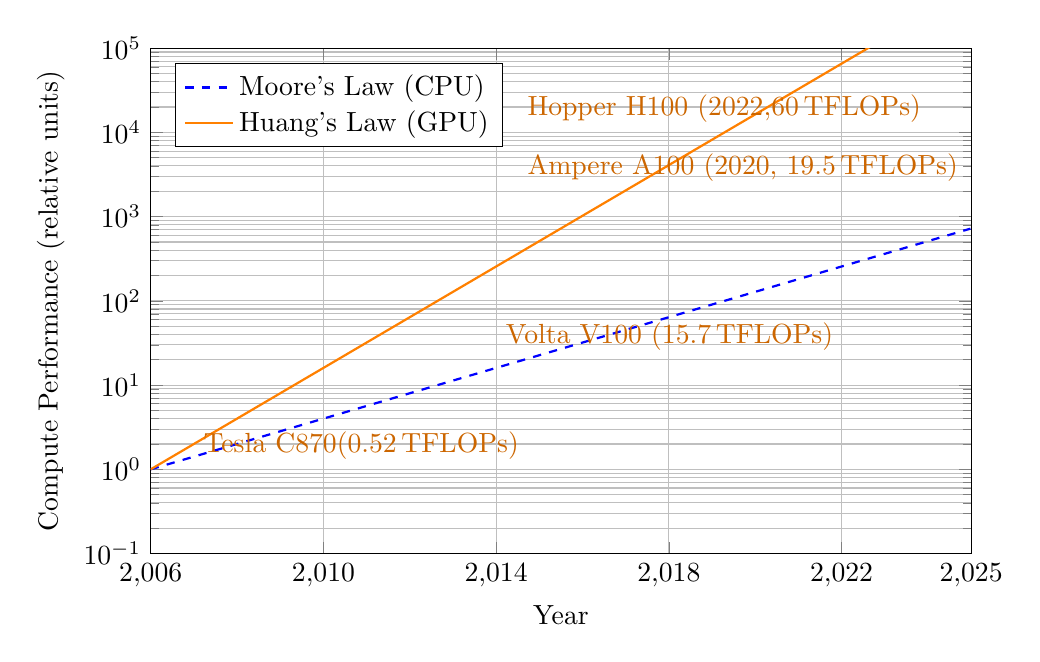
\begin{tikzpicture}
  \begin{semilogyaxis}[
    width=12cm, height=8cm,
    xlabel={Year},
    ylabel={Compute Performance (relative units)},
    xmin=2006, xmax=2025,
    ymin=0.1, ymax=1e5,
    xtick={2006,2010,2014,2018,2022,2025},
    grid=both,
    legend pos=north west,
    legend cell align=left,
    every axis plot/.append style={thick}
  ]

  % Moore's Law (doubling every two years)
  \addplot[
    blue, dashed, domain=2006:2025, samples=200
  ] {2^((x-2006)/2)};
  \addlegendentry{Moore's Law (CPU)}

  % Huang's Law (doubling every year)
  \addplot[
    orange, domain=2006:2025, samples=200
  ] {2^(x-2006)};
  \addlegendentry{Huang's Law (GPU)}

  % GPU Milestones
  \node[anchor=south west,orange!80!black] at (axis cs:2007,1) {Tesla C870(\SI{0.52}{TFLOPs})};
  \node[anchor=south west,orange!80!black] at (axis cs:2014,20) {Volta V100 (\SI{15.7}{TFLOPs})};
  \node[anchor=south west,orange!80!black] at (axis cs:2014.5,2000) {Ampere A100 (2020, \SI{19.5}{TFLOPs})};
  \node[anchor=south west,orange!80!black] at (axis cs:2014.5,10000) {Hopper H100 (2022,\SI{60}{TFLOPs})};
  \end{semilogyaxis}
\end{tikzpicture}

\end{frame}



\begin{frame}[plain,fragile]
\frametitle{Machine learning and AI models are computationally expensive}


% inline figure
\centerline{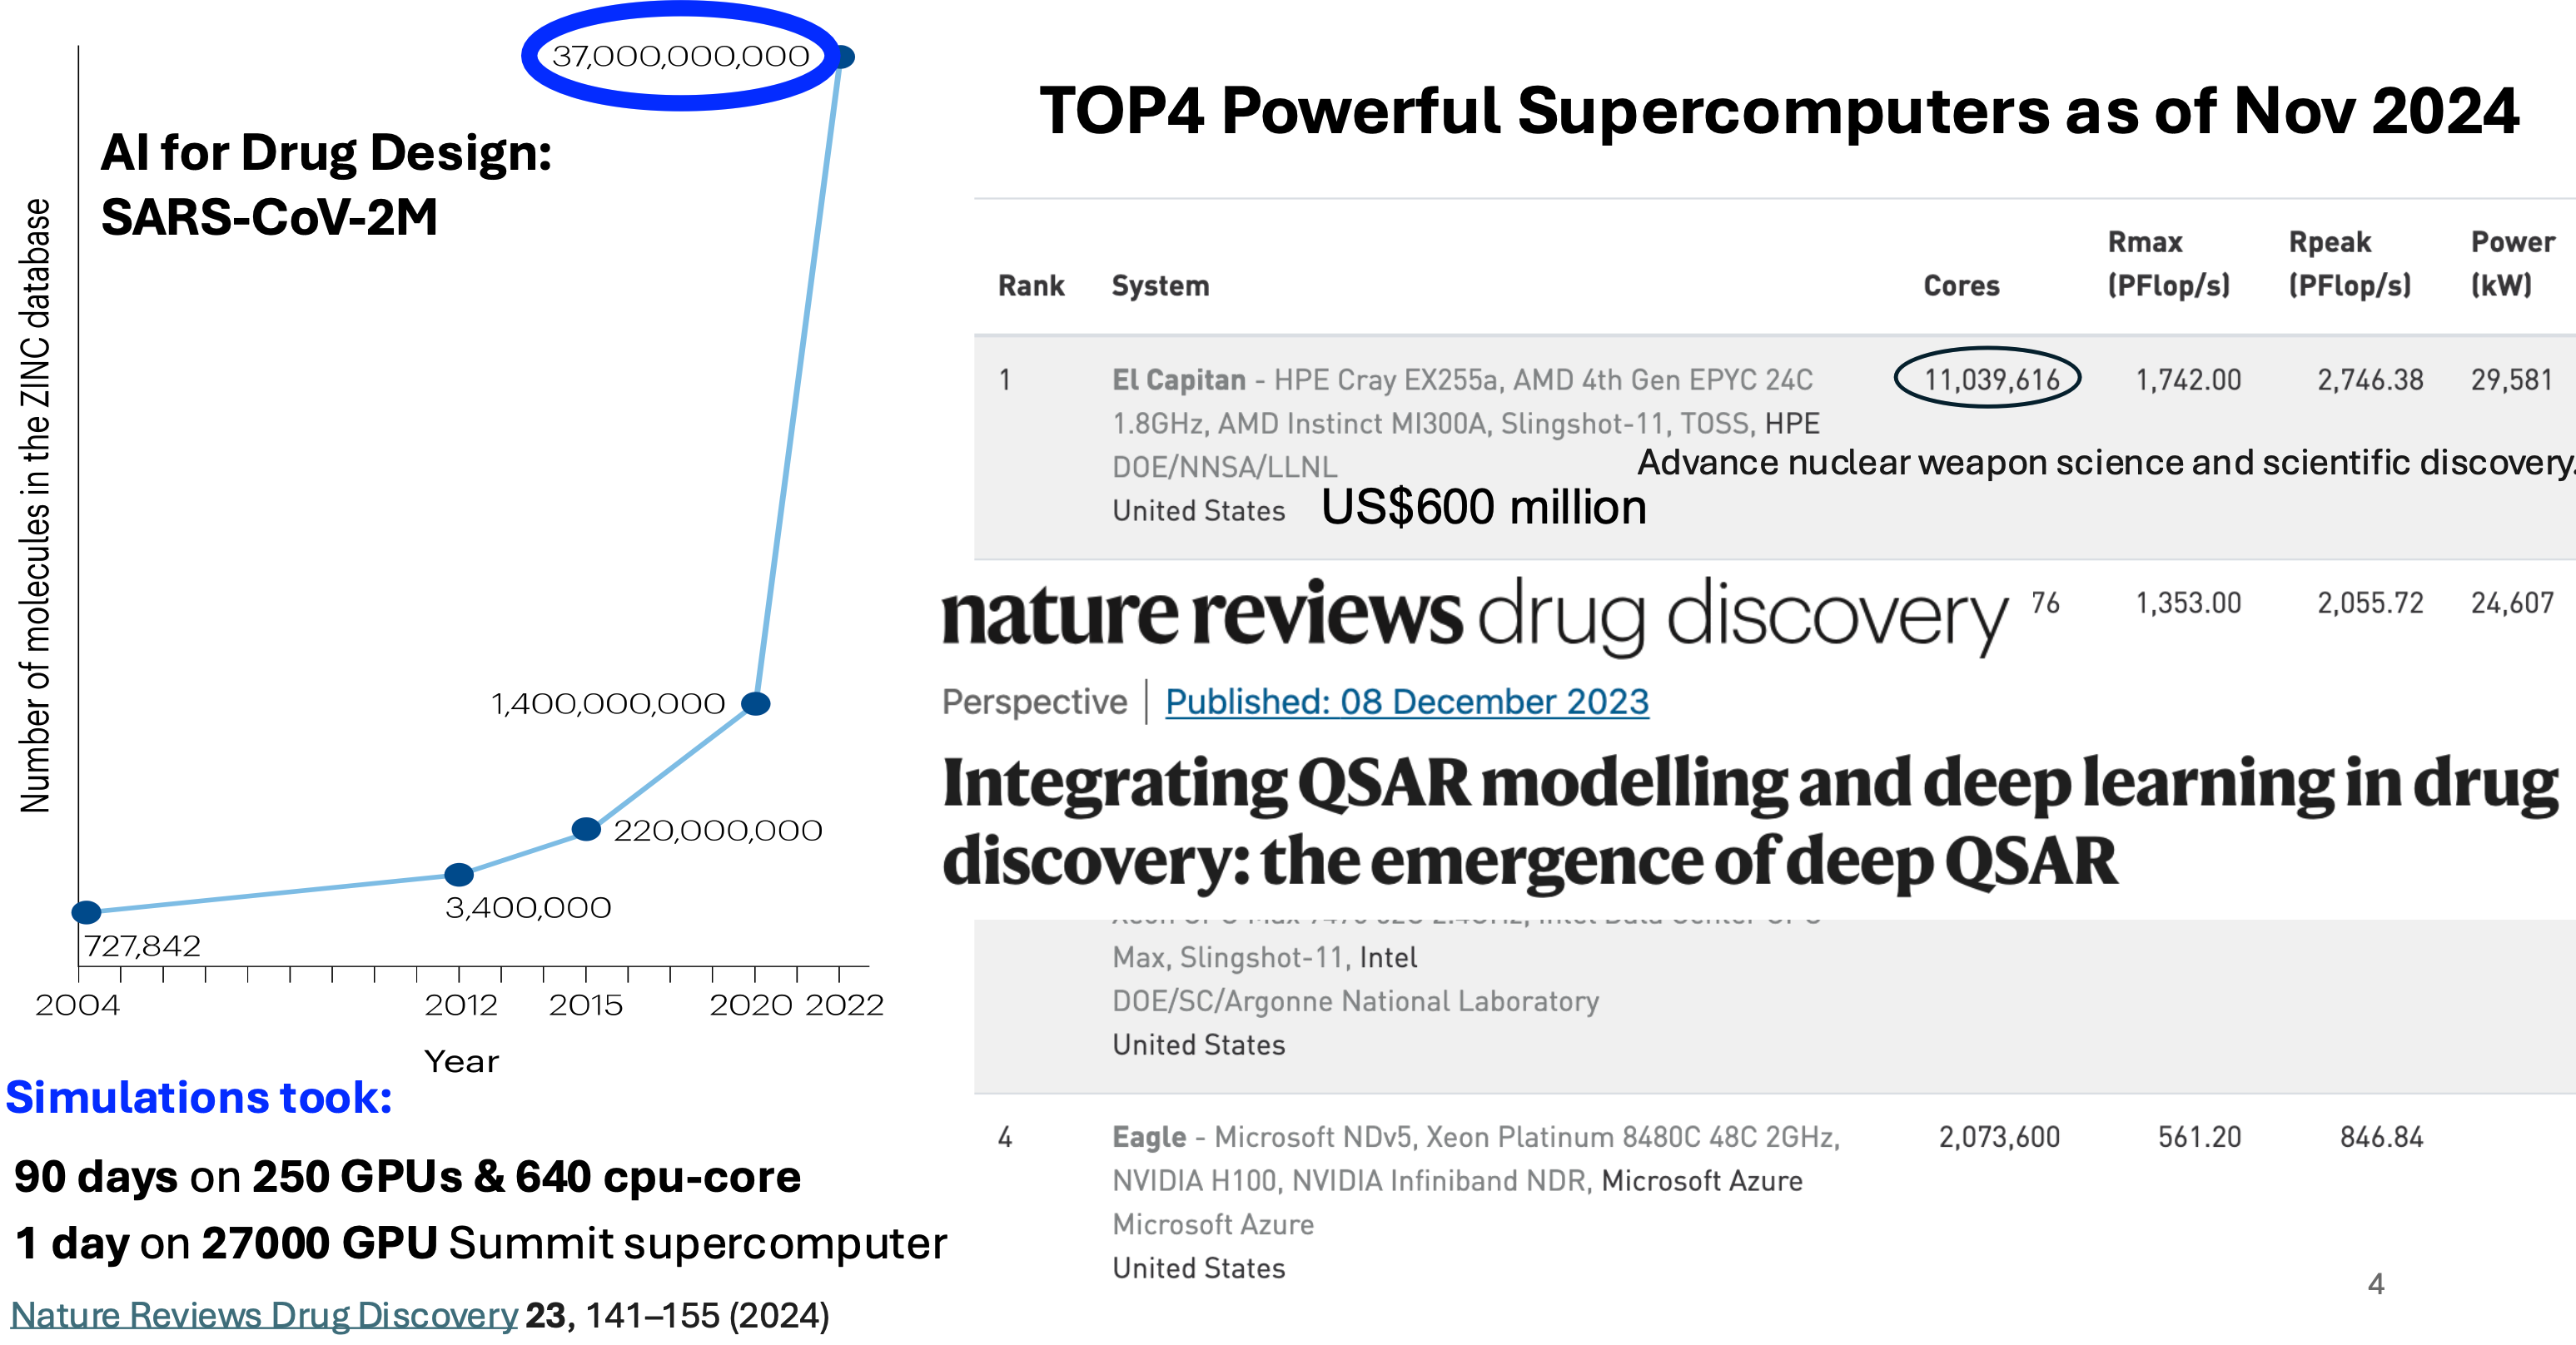
\includegraphics[width=1.0\linewidth]{figures/aitalk2.png}}

\end{frame}


\begin{frame}[plain,fragile]
\frametitle{And power greedy, perhaps quantum computers can reduce the impact?}

% inline figure
\centerline{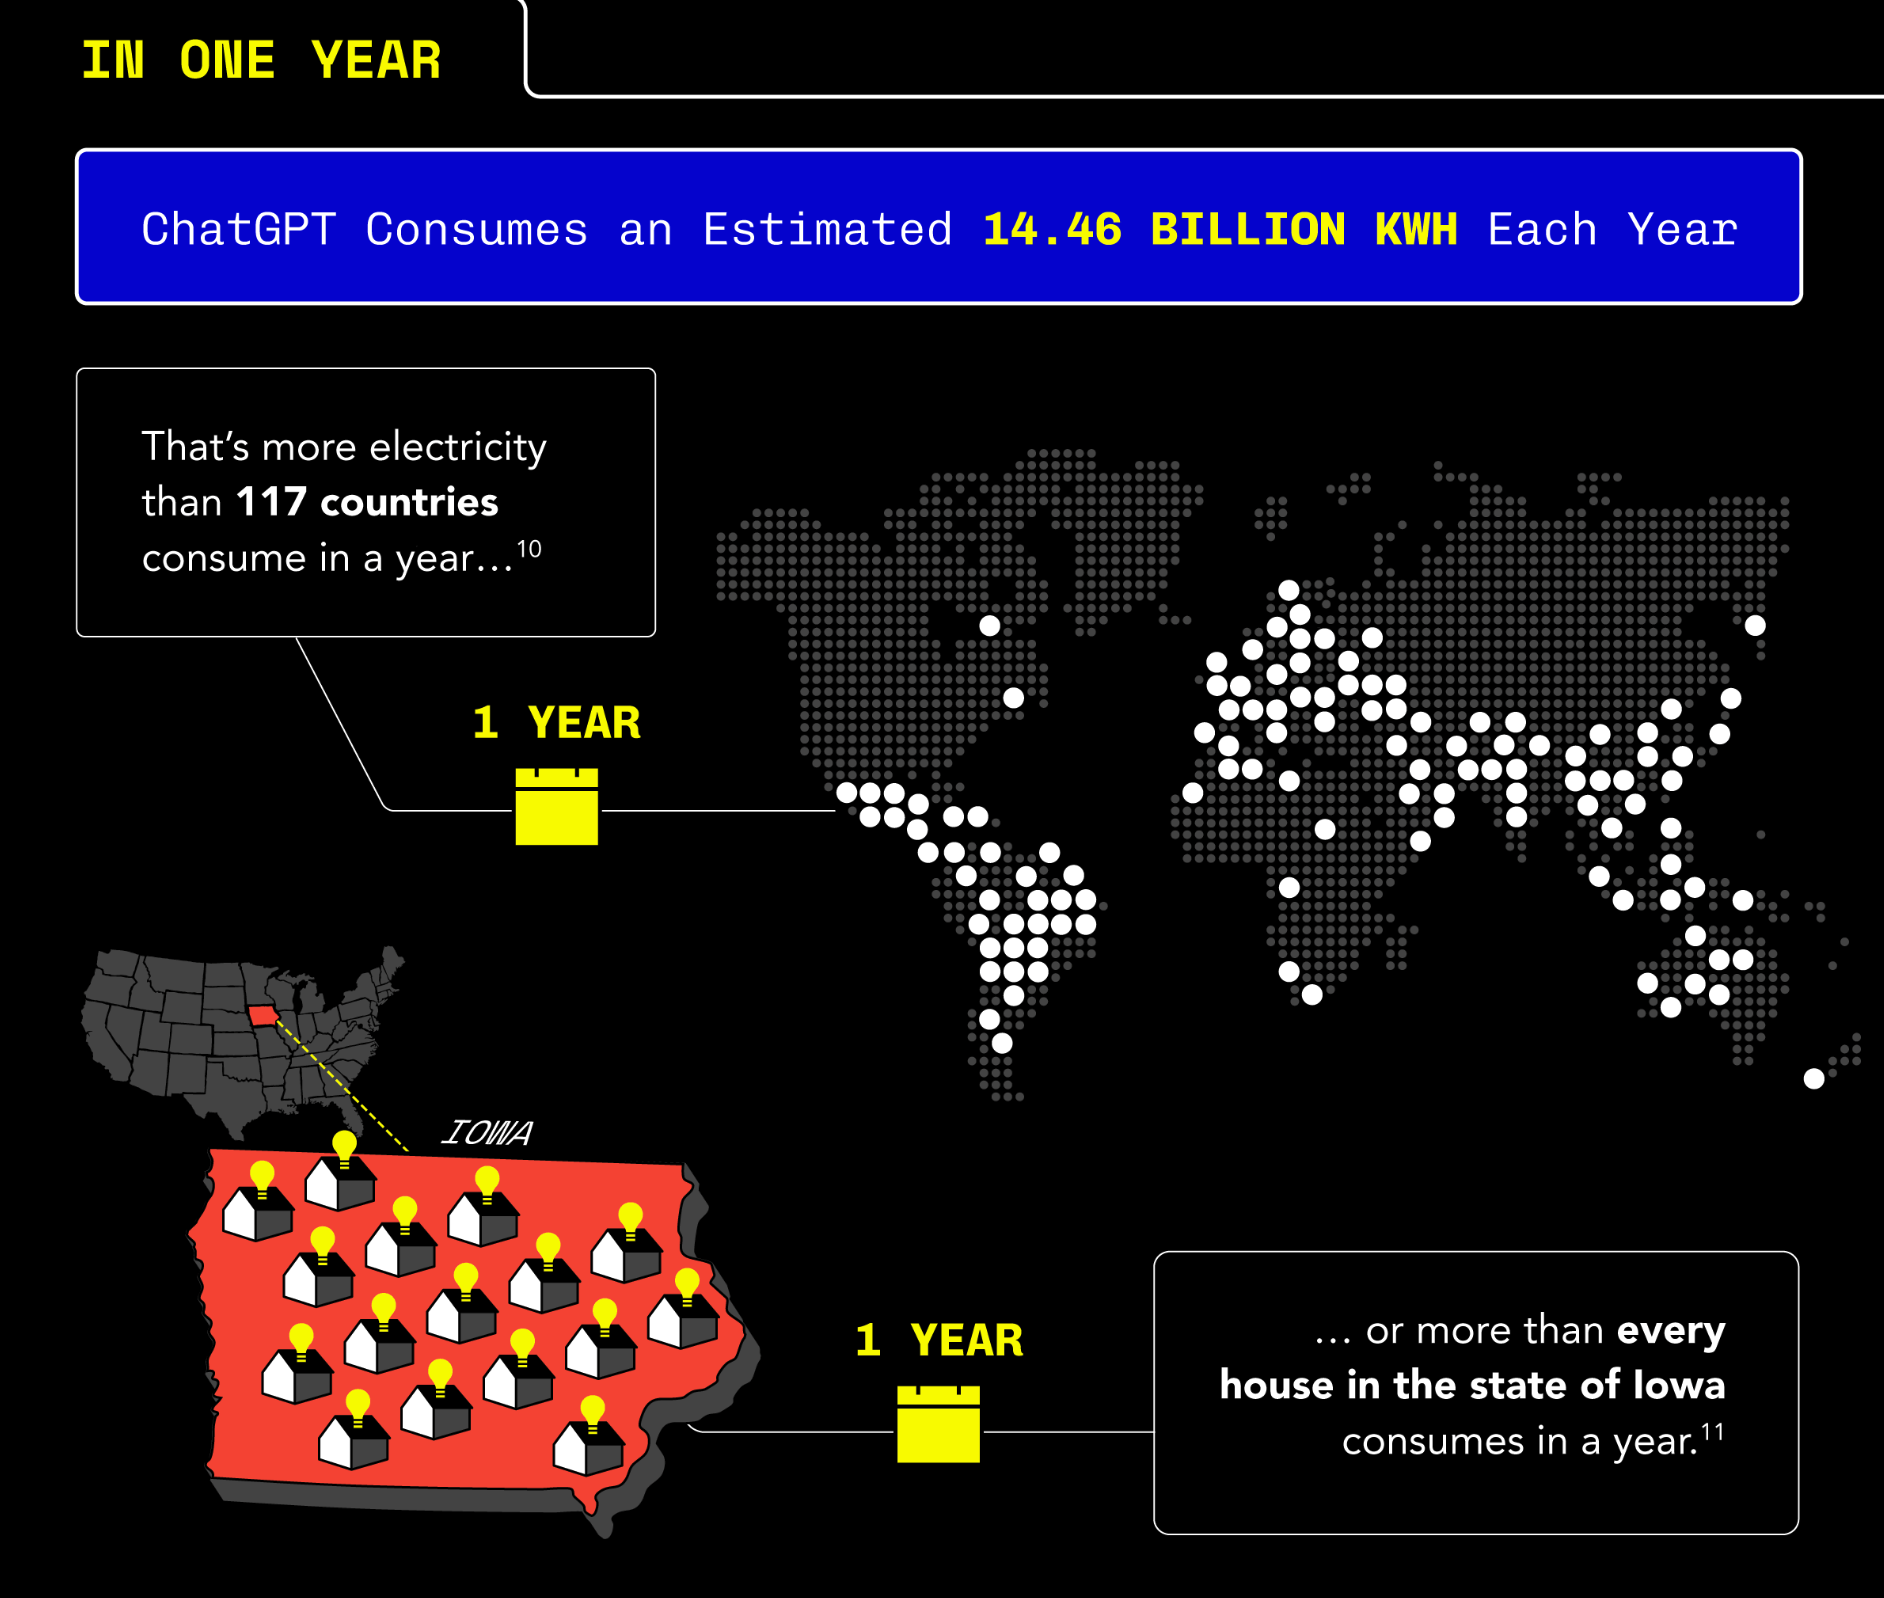
\includegraphics[width=0.7\linewidth]{figures/aitalk1.png}}
Taken from \url{https://www.businessenergyuk.com/knowledge-hub/chatgpt-energy-consumption-visualized/}
\end{frame}

\begin{frame}
\frametitle{And perhaps not environmentally friendly}
\begin{itemize}
\item In Ireland, data centers consume more than 20 percent of the country’s electricity.
\item In Chile, precious aquifers are in danger of depletion.
\item In South Africa, where blackouts have long been routine, data centers are further taxing the national grid.
\item Similar concerns have surfaced in Brazil, Britain, India, Malaysia, the Netherlands, Singapore and Spain and other countries.
\end{itemize}
\end{frame}

\begin{frame}[plain,fragile]
\frametitle{The future is here, sooner than we may think}


% inline figure
\centerline{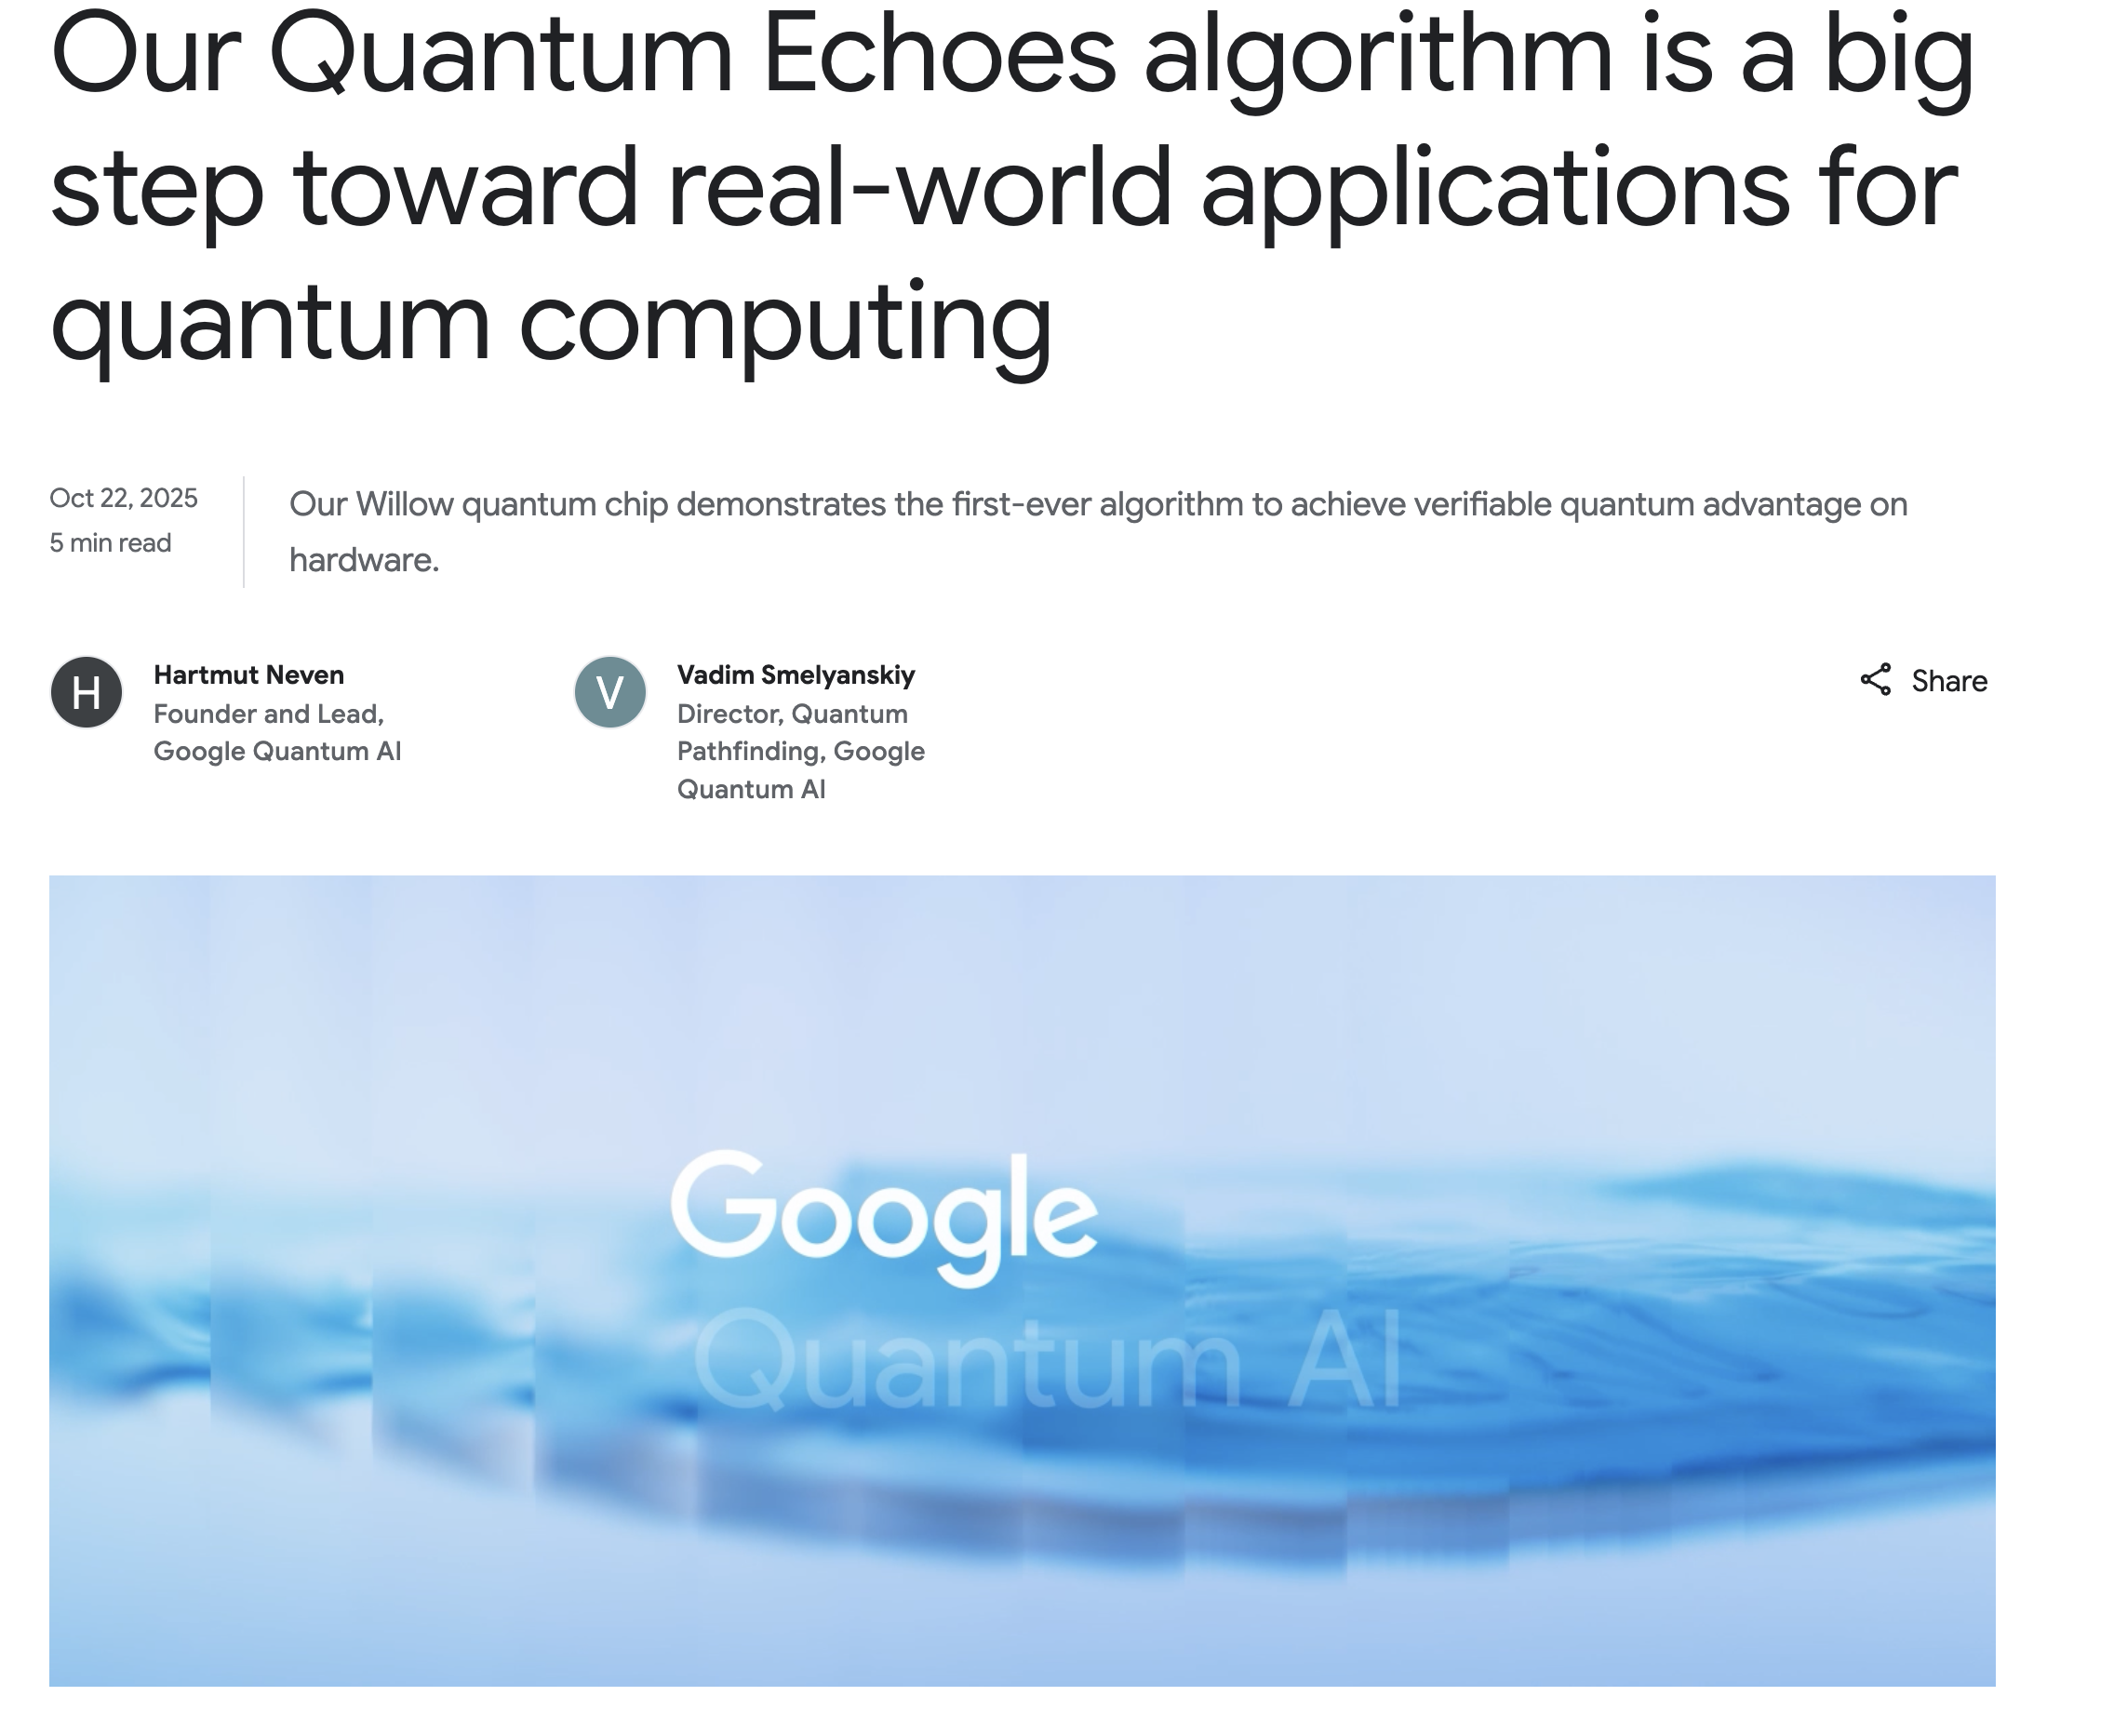
\includegraphics[width=1.05\linewidth]{figures/figuregoogle1.png}}

\end{frame}


\begin{frame}[plain,fragile]
\frametitle{Modern quantum platforms require cooling down to extremely low temperatures}


% inline figure
\centerline{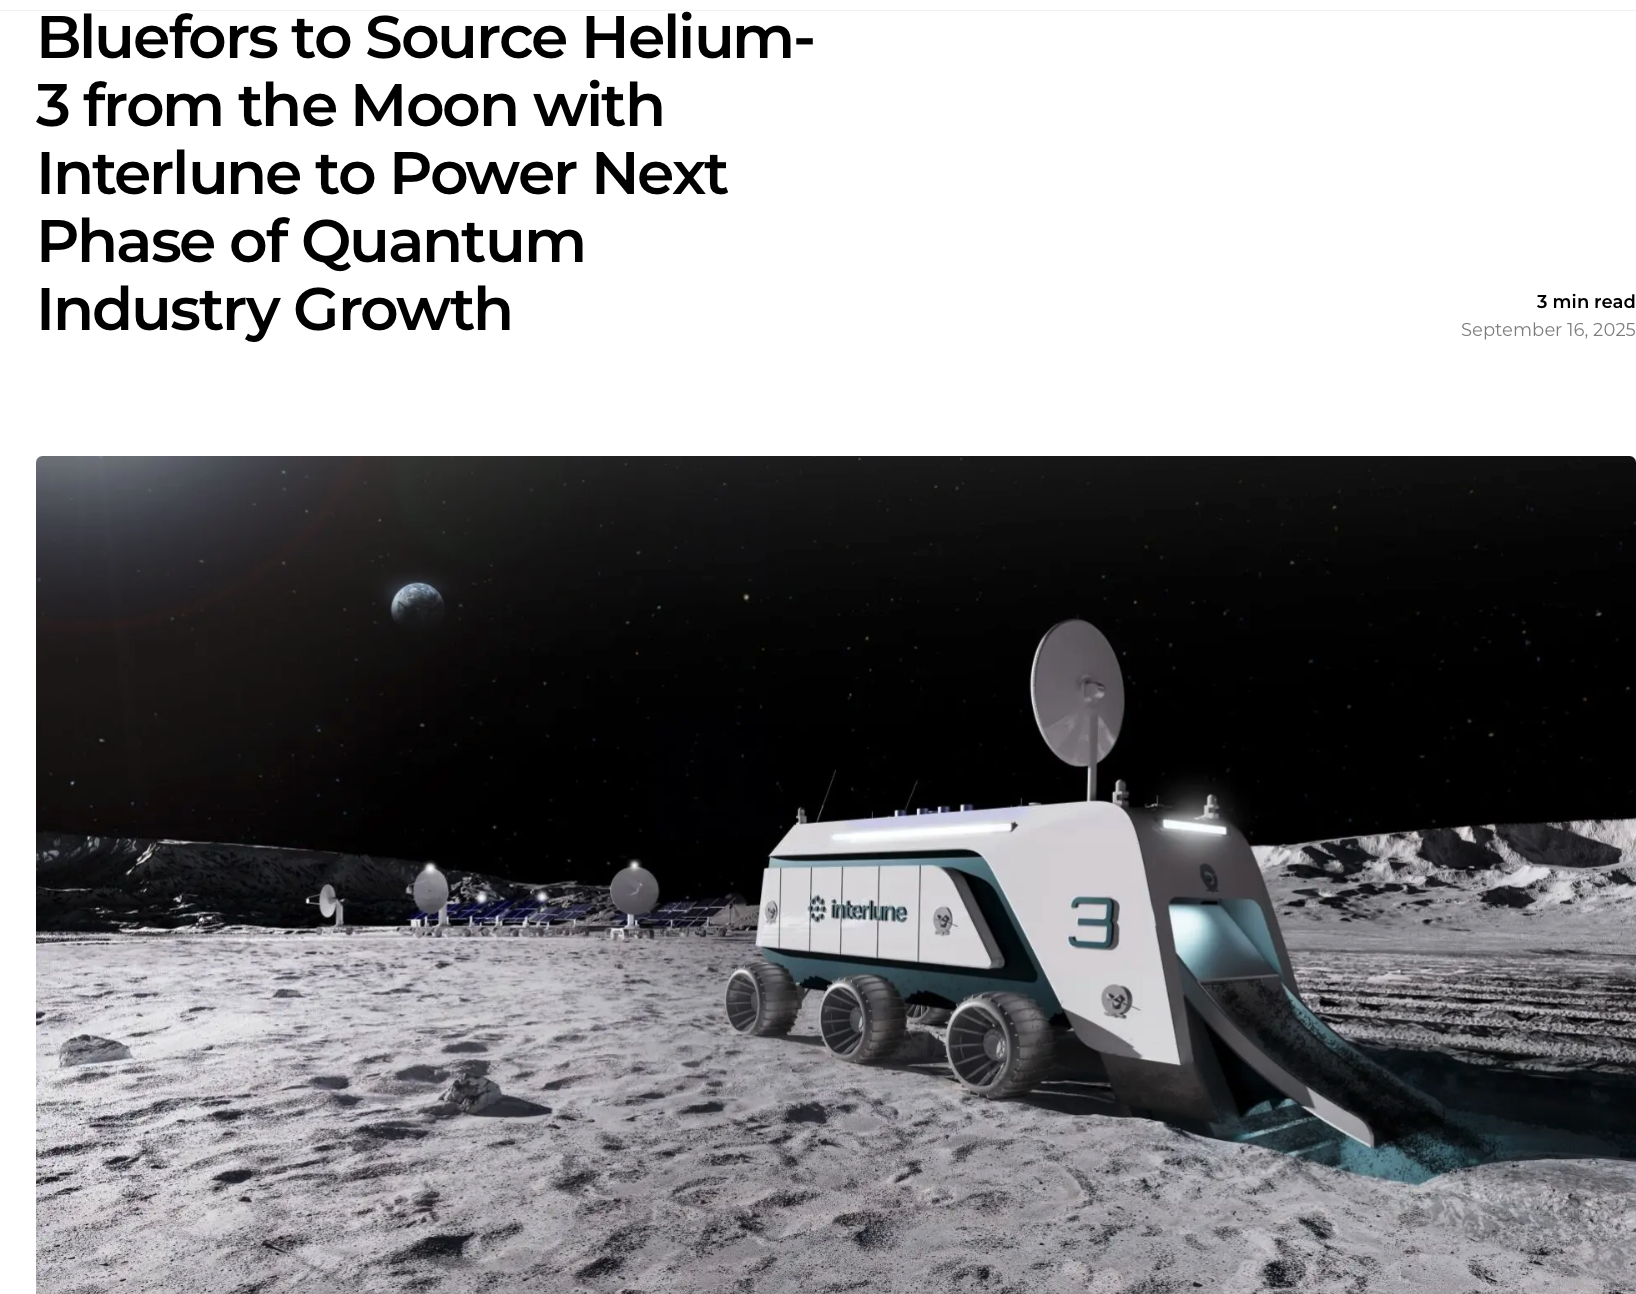
\includegraphics[width=1.05\linewidth]{figures/miningthemoon.png}}

\end{frame}


%\begin{frame}[plain,fragile]
%\frametitle{Add info about tech regulations in AI}
%US-China war on restriciting access to sophisticated technologies
%\begin{enumerate}
%\item TSMC restrictions
%\item Seagate, Micron
%\item Huawei, Nvidia etc, semiconductor control etc
%\end{enumerate}
%Mention Alessandro Aresu's book
%\end{frame}



\begin{frame}{What is quantum technology? Three main fields}
\begin{block}{Quantum computing} is a new computing paradigm that capitalizes on the laws of quantum mechanics to provide significant performance improvement for certain applications, and to enable new territories of computing beyond existing classical
computing.
\end{block}
\begin{block}{Quantum communication} is the secure transfer of quantum information across distances and could ensure security ofcommunication even in the face of unlimited quantum computing power.
\end{block}    
\begin{block}{Quantum sensing} includes a new generation of sensors, based on quantum systems, that provide measurements of various
quantities (for example, electromagnetic fields, gravity, or time) and that are orders of magnitude more sensitive than classical
sensors.
\end{block}
\end{frame}


%-----------------------------------------------------------
%\section{Introduction to Quantum Computing}
\begin{frame}{The basic concepts}
Quantum technologies leverage principles of quantum mechanics to perform computations beyond classical capabilities.

\vspace{10pt}
\textbf{Key Concepts:}
\begin{itemize}
\item \textbf{Superposition:} Qubits can exist in a combination of states.
\item \textbf{Entanglement:} Correlation between qubits regardless of distance.
\item \textbf{Quantum Interference:} Probability amplitudes interfere. Is a core tool in quantum algorithms. It is used to amplify the probability of finding the correct answer while suppressing incorrect ones.
\end{itemize}

\end{frame}

\begin{frame}{Superposition}

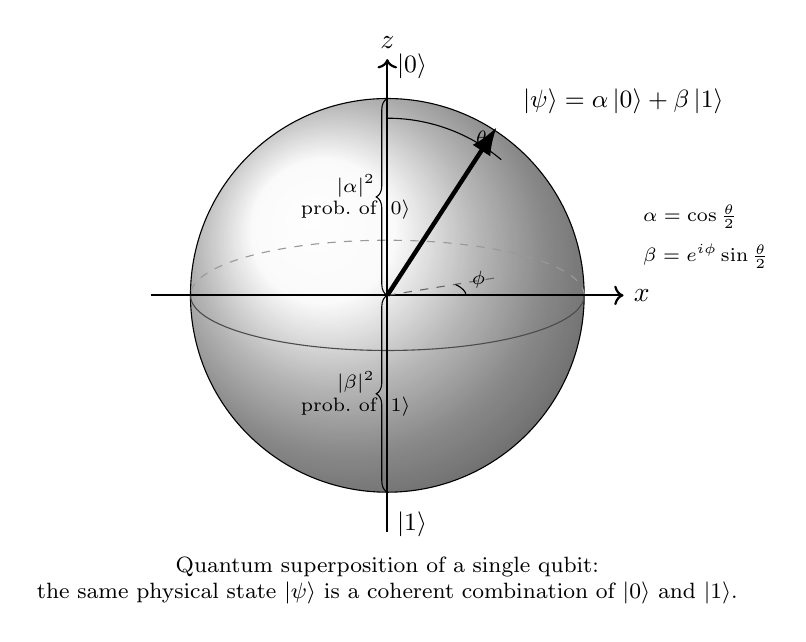
\begin{tikzpicture}[scale=2.5,
   axis/.style={->, thick},
   basislabel/.style={anchor=south east, inner sep=1pt, font=\small},
   statelabel/.style={anchor=west, font=\small},
   myvec/.style={-Latex, thick},
]

% Bloch sphere
\shade[ball color=white!95!gray, opacity=0.9] (0,0) circle (1cm);
\draw[thin, black] (0,0) circle (1cm);

% Draw "equator" ellipse (x-y plane)
\draw[thin, black!70] (-1,0) arc[start angle=180, end angle=360, x radius=1cm, y radius=0.28cm];
\draw[dashed, thin, black!40] (1,0) arc[start angle=0, end angle=180, x radius=1cm, y radius=0.28cm];

% Axes
\draw[axis] (0,-1.2) -- (0,1.2) node[above] {$z$};
\draw[axis] (-1.2,0) -- (1.2,0) node[right] {$x$};

% Poles: |0> at +z, |1> at -z
\node[font=\small, anchor=south west] at (0,1.05) {$\ket{0}$};
\node[font=\small, anchor=north west] at (0,-1.05) {$\ket{1}$};

% State vector |ψ>
% We'll pick some angles θ and φ.
% θ = polar angle from +z, φ = azimuth in x-y plane.
% Say θ = 40°, φ = 30°
\pgfmathsetmacro{\th}{40}   % polar
\pgfmathsetmacro{\ph}{30}   % azimuth
\pgfmathsetmacro{\xp}{sin(\th)*cos(\ph)}
\pgfmathsetmacro{\yp}{0.28*sin(\th)*sin(\ph)} % projected y (ellipse scaling)
\pgfmathsetmacro{\zp}{cos(\th)}

% draw projection of state onto equator
\draw[dashed, black!60] (0,0) -- (\xp,\yp);

% state vector
\draw[myvec, ultra thick] (0,0) -- (\xp,\yp+\zp);

% angle θ from +z axis
\draw[thin] (0,0.9) arc[start angle=90, end angle={90-\th}, radius=0.9cm];
\node[font=\scriptsize, anchor=west] at (0.4,0.8) {$\theta$};

% angle φ in x-y plane
\draw[thin] (0.4,0) arc[start angle=0, end angle=\ph, x radius=0.4cm, y radius=0.11cm];
\node[font=\scriptsize, anchor=west] at (0.38,0.08) {$\phi$};

% Label the state vector
\node[statelabel] at ($(0,0)!1.15!(\xp,\yp+\zp)$) {$\ket{\psi} =
\alpha\ket{0} + \beta\ket{1}$};

% Show alpha,beta magnitudes as cos(θ/2), sin(θ/2)
\node[font=\scriptsize, align=left, anchor=west] at (1.25,0.4) {$\alpha = \cos\frac{\theta}{2}$};
\node[font=\scriptsize, align=left, anchor=west] at (1.25,0.2) {$\beta = e^{i\phi}\sin\frac{\theta}{2}$};

% Little braces showing probabilities
\draw[decorate,decoration={brace, amplitude=4pt}]
 (0,0) -- (0,1)
 node[midway, xshift=-0.4cm, font=\scriptsize, align=center]
 {$|\alpha|^2$\\prob.\ of $\ket{0}$};

\draw[decorate,decoration={brace, amplitude=4pt}]
 (0,-1) -- (0,0)
 node[midway, xshift=-0.4cm, font=\scriptsize, align=center]
 {$|\beta|^2$\\prob.\ of $\ket{1}$};

% Caption under figure
\node[font=\footnotesize, align=center] at (0,-1.45)
{Quantum superposition of a single qubit:\\
the same physical state $\ket{\psi}$ is a coherent combination
of $\ket{0}$ and $\ket{1}$.};

\end{tikzpicture}
\end{frame}


\begin{frame}{What is Quantum Entanglement?}
\textbf{Quantum Entanglement} is a quantum phenomenon where two or more particles become correlated in such a way that the state of one particle directly affects the state of the other, regardless of distance. Fundamental for making quantum gates, quantum sensors and much more. 

\vspace{10pt}
\textbf{Key Features:}
\begin{itemize}
    \item Non-local correlations
    \item No classical analog
\end{itemize}

\end{frame}


\begin{frame}{Entanglement}
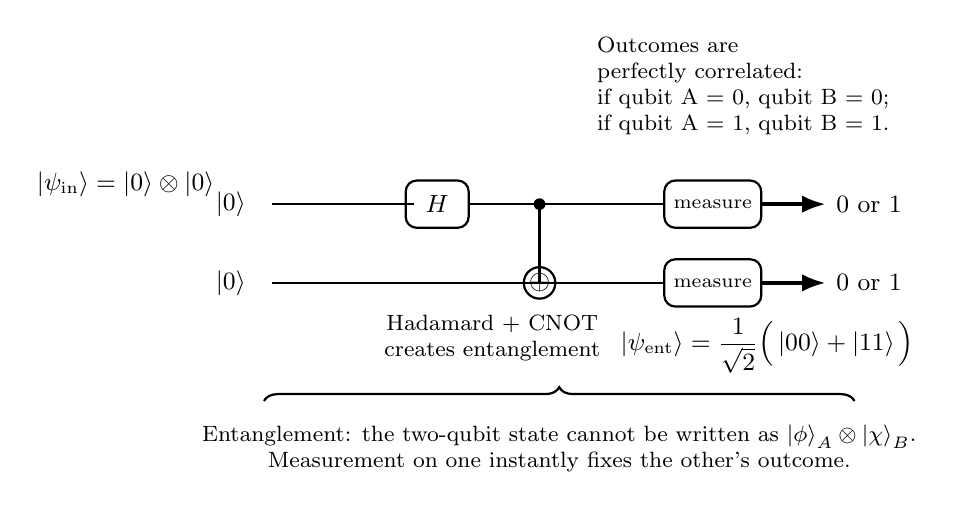
\begin{tikzpicture}[
   thick,
   wire/.style={thick},
   gate/.style={draw, rounded corners, minimum width=0.8cm, minimum height=0.6cm, font=\small, fill=white},
   ctrl/.style={fill=black, circle, inner sep=1.5pt},
   target/.style={draw, circle, inner sep=0pt, minimum width=0.4cm},
   measure/.style={draw, rounded corners, minimum width=0.9cm, minimum height=0.6cm, font=\scriptsize, fill=white},
   amp/.style={-Latex, very thick},
   note/.style={font=\small},
   outcome/.style={font=\small, align=center},
   corr/.style={font=\footnotesize},
]

%%%% 1. LEFT: Initial product state %%%%

\node[note, anchor=east] (psi0label) at (-0.4,0.75)
{$\displaystyle \ket{\psi_\text{in}} = \ket{0}\otimes\ket{0}$};

% Input kets (two wires)
\node[note, anchor=east] (q0in) at (0,0.5) {$\ket{0}$};
\node[note, anchor=east] (q1in) at (0,-0.5) {$\ket{0}$};

% Horizontal wires (input region to circuit region)
\draw[wire] (0.2,0.5) -- (2.0,0.5);
\draw[wire] (0.2,-0.5) -- (2.0,-0.5);

%%%% 2. CIRCUIT: H on top, then CNOT %%%%

% Hadamard gate on first qubit
\node[gate] (Hgate) at (2.3,0.5) {$H$};

\draw[wire] (2.0,0.5) -- (Hgate.west);
\draw[wire] (Hgate.east) -- (3.2,0.5);

% Vertical line for CNOT control-target
\draw[wire] (3.6,0.5) -- (3.6,-0.5);

% Control dot on top wire
\node[ctrl] (ctrl) at (3.6,0.5) {};

% Target ⊕ on bottom wire
\node[target] (targ) at (3.6,-0.5) {$\oplus$};

% extend wires to the right of CNOT
\draw[wire] (3.2,0.5) -- (4.2,0.5);
\draw[wire] (2.0,-0.5) -- (4.2,-0.5);

% Label under circuit: "Entangling operation"
\node[font=\footnotesize, align=center] at (3.0,-1.2)
{Hadamard + CNOT\\creates entanglement};

%%%% 3. STATE AFTER CIRCUIT %%%%

\node[note, anchor=west] (psiBell) at (4.5,-1.3)
{$\displaystyle
\ket{\psi_\text{ent}} =
\frac{1}{\sqrt{2}}\Big(\ket{00}+\ket{11}\Big)
$};

%%%% 4. MEASUREMENT BOXES %%%%

% Measurement boxes on each qubit
\node[measure] (M0) at (5.8,0.5) {measure};
\node[measure] (M1) at (5.8,-0.5) {measure};

% wires into measurement
\draw[wire] (4.2,0.5) -- (M0.west);
\draw[wire] (4.2,-0.5) -- (M1.west);

% classical arrows out
\draw[amp] (M0.east) -- ++(0.8,0.0) node[outcome, anchor=west]
{$0$ or $1$};
\draw[amp] (M1.east) -- ++(0.8,0.0) node[outcome, anchor=west]
{$0$ or $1$};

% Correlation annotation
\node[corr, align=left, anchor=west] at (4.2,2.0)
{Outcomes are\\perfectly correlated:\\
if qubit A = 0, qubit B = 0;\\
if qubit A = 1, qubit B = 1.};

%%%% 5. BIG BRACE + TEXT EXPLANATION %%%%

% Decorative brace under entire figure
\draw[decorate, decoration={brace, amplitude=5pt}]
 (0.1,-2.0) -- (7.6,-2.0)
 node[midway, yshift=-0.6cm, align=center, font=\footnotesize]
 {Entanglement: the two-qubit state cannot be written
  as $\ket{\phi}_A \otimes \ket{\chi}_B$.\\
  Measurement on one instantly fixes the other's outcome.};

\end{tikzpicture}
\end{frame}







\begin{frame}{Quantum Speedups}
\textbf{Why Quantum?}
\begin{itemize}
    \item \textbf{Quantum Parallelism:} Process multiple states simultaneously.
    \item \textbf{Quantum Entanglement:} Correlated states for richer information.
    \item \textbf{Quantum Interference:} Constructive and destructive interference to enhance solutions, is a core tool in quantum algorithms. 
\end{itemize}

\textbf{Example - Grover's Algorithm:}
\[
\text{Quantum Search Complexity: } O(\sqrt{N}) \text{ vs. } O(N)
\]

\textbf{Advantage:}
- Speedups in high-dimensional optimization and linear algebra problems.
\end{frame}

%-----------------------------------------------------------
%\section{Challenges in Quantum Machine Learning}
\begin{frame}{Challenges and Limitations}
\textbf{1. Quantum Hardware Limitations:}
\begin{itemize}
    \item Noisy Intermediate-Scale Quantum (NISQ) devices.
    \item Decoherence and limited qubit coherence times.
\end{itemize}

\textbf{2. Data Encoding:}
\begin{itemize}
    \item Efficient embedding of classical data into quantum states.
\end{itemize}

\textbf{3. Scalability:}
\begin{itemize}
    \item Difficult to scale circuits to large datasets.
\end{itemize}
\end{frame}






\begin{frame}{1. Quantum Communication}
\textbf{Quantum Teleportation:}
\begin{itemize}
    \item Entanglement enables the transmission of quantum states using classical communication.
    \item No need to send the physical quantum particle.
\end{itemize}

\textbf{Advantage:}
\begin{itemize}
\item Instantaneous state transfer within quantum mechanics constraints.
\item Quantum networks rely on entanglement for secure communication.
  \end{itemize}
\end{frame}

\begin{frame}{2. Quantum Cryptography}
\textbf{Quantum Key Distribution:}
\begin{itemize}
    \item Entanglement ensures secure communication.
    \item Eavesdropping disturbs quantum states, revealing interception attempts.
\end{itemize}

\begin{itemize}
\item Any measurement by a third party collapses the wavefunction.  
\item Ensures security based on quantum mechanics, not computational hardness.
\end{itemize}
\textbf{Advantage:} Unconditional security guaranteed by the laws of physics.
\end{frame}

\begin{frame}{3. Quantum Computing}
\textbf{Speedup in Quantum Algorithms:}
\begin{itemize}
    \item Entanglement provides exponential state space.
    \item Quantum parallelism arises from entangled qubits.
\end{itemize}

\textbf{Grover's Algorithm:}
\[
\mathcal{O}(\sqrt{N}) \text{ vs. } \mathcal{O}(N)
\]

\textbf{Shor's Algorithm:}
\[
\text{Factoring in } \mathcal{O}((\log N)^3)
\]
\end{frame}

\begin{frame}[plain,fragile]
\frametitle{4. Quantum Metrology}

\textbf{Quantum Metrology:}
\begin{itemize}
    \item Uses entangled states for ultra-precise measurements.
    \item Overcomes the classical shot-noise limit.
\end{itemize}

\textbf{Heisenberg Limit:}
\[
\Delta \theta \ge \frac{1}{N},
\]

where \( N \) is the number of entangled particles.  

\begin{block}{Advantage:}
\begin{itemize}
\item Quantum entanglement improves sensitivity beyond classical limits.
\end{itemize}
\end{block}
\end{frame}

\begin{frame}{Challenges of Quantum Entanglement}
\textbf{Decoherence:}
\begin{itemize}
    \item Entangled states are fragile.
    \item Interaction with the environment collapses the wavefunction.
\end{itemize}

\textbf{Scalability:}
\begin{itemize}
    \item Difficult to entangle large numbers of qubits.
    \item Error correction requires complex protocols.
\end{itemize}

\textbf{Measurement Problem:}
\begin{itemize}
    \item Measurement destroys entanglement.
    \item Trade-off between information gain and entanglement preservation.
\end{itemize}
\end{frame}

%-----------------------------------------------------------
%\section{Quantum Machine Learning (QML)}
\begin{frame}{What is Quantum Machine Learning?}
\textbf{Quantum Machine Learning (QML)} integrates quantum computing with machine learning algorithms to exploit quantum advantages.

\vspace{10pt}
\textbf{Motivation:}
\begin{itemize}
    \item High-dimensional Hilbert spaces for better feature representation.
    \item Quantum parallelism for faster computation.
    \item Quantum entanglement for richer data encoding.
\end{itemize}


\end{frame}



\begin{frame}[plain,fragile]
\frametitle{Di Vincenzo criteria}

\begin{alertblock}{Quantum computing requirements}
\begin{enumerate}
\item A scalable physical system with well-characterized qubit

\item The ability to initialize the state of the qubits to a simple fiducial state

\item Long relevant Quantum coherence times longer than the gate operation time

\item A \textbf{universal} set of quantum gates

\item A qubit-specific measurement capability
\end{enumerate}

\noindent
\end{alertblock}
\end{frame}

\begin{frame}[plain,fragile]
\frametitle{Quantum platforms}

\begin{enumerate}
\item Superconducting qubits use Josephson junction circuits operated at millikelvin temperatures
\item Trapped-ion computers confine ions (e.g.\ $^{171}$Yb$^+$, $^{40}$Ca$^+$) in electromagnetic traps, encoding qubits in internal electronic states. Gates are implemented with laser or microwave fields coupling to vibrational modes.
\item Photonic quantum computing employs photons (in dual-rail or  continuous-variable encodings) as qubits
\item Spin qubits—realized in silicon quantum dots, donor atoms, or color centers—encode information in electron or nuclear spin states.
  \item Electrons on helium/neon (more on this below, own research)

\end{enumerate}


\end{frame}



\section{The next decade}

\begin{frame}[plain,fragile]
\frametitle{Considerable investements (McKinsey Quantum Technology Monitor, June 2025 )}


% inline figure
\centerline{
\includegraphics[width=0.9\linewidth]{qcfigures/image1.png}}

\end{frame}


\begin{frame}[plain,fragile]
\frametitle{Quantum technology (QT) investments by funding type, 2014–24}


% inline figure
\centerline{
\includegraphics[width=0.9\linewidth]{qcfigures/image2.png}}

\end{frame}

\begin{frame}[plain,fragile]
\frametitle{Announcements of public investments in quantum technology }


% inline figure
\centerline{
\includegraphics[width=0.9\linewidth]{qcfigures/image3.png}}

\end{frame}

\begin{frame}[plain,fragile]
\frametitle{The United States and Japan lead other countries in the number of patents
granted for quantum technology}


% inline figure
\centerline{
\includegraphics[width=1.0\linewidth]{qcfigures/image4.png}}

\end{frame}

\begin{frame}[plain,fragile]
\frametitle{The United States and China lead other countries in the number of filed patents}


% inline figure
\centerline{
\includegraphics[width=1.0\linewidth]{qcfigures/image5.png}}

\end{frame}


\begin{frame}[plain,fragile]
\frametitle{The quantum communication market is projected to reach 11 billion to
15 billion USD by 2035.}


% inline figure
\centerline{
\includegraphics[width=0.9\linewidth]{qcfigures/image6.png}}

\end{frame}



    

\section{Legal aspects and export control resrictions}



\frame
    {
      \frametitle{New platform: electrons on helium, \url{https://eeroq.com/}}

      \begin{footnotesize}
     \begin{columns}
       \column{5.0cm}
\begin{enumerate}
\item Long coherence times

\item Highly connected qubits

\item Many and controllable qubits in a small area

\item CMOS compatible

\item Fast gates
\end{enumerate}

\column{6cm}
      \begin{center}
        \rotatebox[origin=c]{-90}{
\includegraphics[width=1.3\textwidth]{qcfigures/lab.jpeg}}
      \end{center}
\end{columns}
      \end{footnotesize}
    }





\frame
    {
      \frametitle{Single electrons can make great qubits}
	
      \begin{footnotesize}
     \begin{columns}
       \column{5.0cm}

       At the heart is the trapping and control
       of individual electrons floating above pools of superfluid
       helium. These electrons form the qubits of our quantum
       computer, and the purity of the superfluid helium protects the
       intrinsic quantum properties of each electron. The  ultimate
       goal is to build a large-scale quantum computer based on
       quantum magnetic (spin) state of these trapped electrons.
\column{5cm}
      \begin{center}
	
\includegraphics[width=1.2\textwidth]{qcfigures/nordicquantumfig1.png}
      \end{center}
\end{columns}
      \end{footnotesize}
    }


\frame
    {
      \frametitle{Trapping electrons in microchannels}
	
      \begin{footnotesize}
     \begin{columns}
       \column{5.0cm}
Microchannels fabricated into silicon wafers are filled with superfluid helium and energized electrodes. Together with the natural electron trapping properties of superfluid helium, these allow for the precision trapping of individual or multiple electrons. The microchannels are only a few micrometers in size, or about five times smaller than the diameter of a human hair.
\column{5cm}
      \begin{center}
	
\includegraphics[width=1.2\textwidth]{qcfigures/nordicquantumfig2.png}
      \end{center}
\end{columns}
      \end{footnotesize}
    }

\frame
    {
      \frametitle{Control and readout}
	
      \begin{footnotesize}
     \begin{columns}
       \column{5.0cm}

       Microchannel regions can store thousands of electrons, from which one can be plucked and transported to the single electron control and readout area. In this region, microwave signals will interact with the electron to perform quantum logic gate operations, which will be readout via extremely fast electronics.


\column{5cm}
      \begin{center}
	
\includegraphics[width=1.2\textwidth]{qcfigures/nordicquantumfig3.png}
      \end{center}
\end{columns}
      \end{footnotesize}
    }


\frame
    {
      \frametitle{Operations for quantum computing}
	
      \begin{footnotesize}
     \begin{columns}
       \column{5.0cm}
Quantum information can be encoded in a number of ways using single electrons. Currently, we are working with the side-to-side(lateral) quantum motion of the electron in the engineered trap. This motion can either be in its lowest energy state, the ground state, or in a number of higher-energy excited states. This electron motion also provides the readout capabilities for the ultimate goal of building a large-scale quantum computer based on the electron's magnetic moment (spin).       
\column{5cm}
      \begin{center}
	
\includegraphics[width=1.2\textwidth]{qcfigures/nordicquantumfig4.png}
      \end{center}
\end{columns}
      \end{footnotesize}
    }
    
\begin{frame}[plain,fragile]
\frametitle{New export control rules}
\begin{block}{}
The US Bureau of Industry and Security (BIS) rules are new export
controls on certain quantum computing items, implemented through an
Interim Final Rule (IFR) on September 6, 2024. These rules add
worldwide licensing requirements for items on the Commerce Control
List (CCL), create a new license exception for allied countries, and
establish reporting requirements. The aim is to control the export of
advanced technologies, including quantum computing components,
software, and equipment, for national security and foreign policy
reasons.
\end{block}

\end{frame}


\begin{frame}[plain,fragile]
\frametitle{What is controlled}
\begin{block}{}
\begin{itemize}
\item Quantum computing items: This includes computers, software, components, materials, and related equipment used in their development and maintenance.
\item Advanced semiconductor manufacturing equipment: Tools and machines for producing advanced chips.
\item Technology: Technology for high-performance computing chips.
Additive manufacturing items: Equipment for producing metal components.
\end{itemize}
\end{block}

\end{frame}




\begin{frame}[plain,fragile]
\frametitle{Export control, selected list from own collaborations}
\begin{block}{Technology/Component and Reason for Sensitivity}
\begin{itemize}
\item Superconducting CPW resonator: Advanced quantum sensor with potential defense/communications applications.
\item Single-electron trap (gated microchannel): Specialized microelectronic architecture for quantum computing. 
\item Superconducting electrodes (Nb films):  Superconducting materials in high-Q resonators and quantum circuits. 
\item Superfluid $^4$He substrate:  Specialized cryogenic environment and novel quantum materials. 
\item Cryogenic RF components:  Similar hardware is used in radar and communications systems.
\item Electron-on-helium qubit platform: Emerging quantum information platform targeted by new export controls; potential secure/advanced computation application. 
\end{itemize}
\end{block}
\end{frame}

\begin{frame}[plain,fragile]
\frametitle{Instead of conclusions: Other topics to discuss}
\begin{itemize}
\item Quantum Technologies and International Treaties
\item Quantum computing raises questions about whether existing statutes on intellectual property, liability, privacy, and even antitrust are adequate 
\item Cybersecurity in the Quantum Era: Threats and Legal Responses – How quantum computing jeopardizes current cryptography and what laws can do about it
\item Quantum Communication and Privacy
\item Quantum Sensing and Surveillance: Privacy and  National Security Implications
\item Export Controls and Quantum Tech: Balancing Security and Innovation
\item Patents and IP in the Quantum Era: Innovation vs. Open Science
\item Geopolitics of Quantum: The New Tech Arms Race and Legal Strategy
\item Ethical Quantum Technologies: Ensuring Responsible Innovation and many more
\end{itemize}

\end{frame}



\end{document}



The US Bureau of Industry and Security (BIS) rules are new export
controls on certain quantum computing items, implemented through an
Interim Final Rule (IFR) on September 6, 2024. These rules add
worldwide licensing requirements for items on the Commerce Control
List (CCL), create a new license exception for allied countries, and
establish reporting requirements. The aim is to control the export of
advanced technologies, including quantum computing components,
software, and equipment, for national security and foreign policy
reasons.

Key aspects of the new rules



Key aspects of the new rules
Worldwide licensing: The controls apply to exports to all destinations, not just those restricted by the Country Chart.
License exception: A new exception, known as License Exception IEC, allows for exports to countries that have implemented equivalent controls, such as Italy, Canada, and the United Kingdom.
Control policy:There is a presumption of approval for exports to Country Group A:1 countries.There is a presumption of denial for exports to Country Groups D:1 and D:5 (such as China and Russia).Case-by-case reviews will be conducted for other countries.
Reporting requirements:
Companies must submit annual reports on certain exports and deemed exports, with a first report deadline of November 5, 2024, for the period of September 6 to October 28, 2024.
Termination reports are required within 30 days of an employee's or contractor's departure in certain situations.  

What is controlled?
Quantum computing items: This includes computers, software, components, materials, and related equipment used in their development and maintenance.
Advanced semiconductor manufacturing equipment: Tools and machines for producing advanced chips.
Gate All-Around Field-Effect Transistor (GAAFET) Technology: Technology for high-performance computing chips.
Additive manufacturing items: Equipment for producing metal components.



\begin{frame}[plain,fragile]
\frametitle{Observations (or conclusions if you prefer)}


\begin{block}{}
\begin{itemize}
\item How do we develop insights, competences, knowledge in AI and quantum technologies  that can advance a given field?
\begin{itemize}

  \item For example: Can we use ML to find out which correlations are relevant and thereby diminish the dimensionality problem in complex interacting  many-particle systems?

  \item Can we use AI/ML in detector analysis, accelerator design, analysis of experimental data and more?

  \item Can we use AL/ML to carry out reliable extrapolations by using current experimental knowledge and current theoretical models?
\item How do we study entanglement in various quantum platforms? Can we use AI/ML for better design?

\end{itemize}

\noindent
\item The community needs to invest in relevant educational efforts and training of scientists with knowledge in AI/ML and quantum technologies

\item Most likely tons of things I have forgotten
\end{itemize}

\noindent
\end{block}
\end{frame}

\begin{frame}{More conclusions or perspectives: Selected applications of Quantum Machine Learning}
\textbf{1. Quantum mechanical many-particle systems:}
\begin{itemize}
    \item Simulate  structures in nuclei, atoms, moleculs etc with QML.
\end{itemize}

\textbf{2. Finance:}
\begin{itemize}
    \item Quantum optimization for portfolio management.
\end{itemize}

\textbf{3. Image Recognition:}
\begin{itemize}
    \item Quantum-enhanced convolutional neural networks.
\end{itemize}
\end{frame}


\begin{frame}[plain,fragile]
\frametitle{Thank you for the attention and results from references in slides)}
\begin{enumerate}

\item Bryce Fore, Jane Kim, Morten Hjorth-Jensen, Alessandro Lovato, \textbf{Investigating the crust of neutron stars with neural-network quantum states}, Communications Physics \textbf{8}, 108  (2025) and \href{{https://www.nature.com/articles/s42005-025-02015-2}}{\nolinkurl{https://www.nature.com/articles/s42005-025-02015-2}}

\item Patrick Cook, Danny Jammooa, Morten Hjorth-Jensen, Daniel D. Lee, Dean Lee, \textbf{Parametric Matrix Models}, Nature Communications  under review and \href{{https://arxiv.org/abs/2401.11694}}{\nolinkurl{https://arxiv.org/abs/2401.11694}}

\item Niyaz R. Beysengulov, Johannes Pollanen, Øyvind S. Schøyen, Stian D. Bilek, Jonas B. Flaten, Oskar Leinonen, Håkon Emil Kristiansen, Zachary J. Stewart, Jared D. Weidman, Angela K. Wilson, Morten Hjorth-Jensen, Coulomb interaction-driven entanglement of electrons on helium, PRX Quantum 5, 030324 (2024) and \href{{https://journals.aps.org/prxquantum/abstract/10.1103/PRXQuantum.5.030324}}{\nolinkurl{https://journals.aps.org/prxquantum/abstract/10.1103/PRXQuantum.5.030324}}

\end{enumerate}
\end{frame}



\begin{frame}[plain,fragile]
\frametitle{Additional references)}
\begin{enumerate}

\item Jane Kim, Gabriel Pescia, Bryce Fore, Jannes Nys, Giuseppe Carleo, Stefano Gandolfi, Morten Hjorth-Jensen, Alessandro Lovato, \textbf{Neural-network quantum states for ultra-cold Fermi gases}, Communications Physics \textbf{7}, 148 (2024) and \href{{https://www.nature.com/articles/s42005-024-01613-w}}{\nolinkurl{https://www.nature.com/articles/s42005-024-01613-w}}

\item Bryce Fore, Jane M. Kim, Giuseppe Carleo, Morten Hjorth-Jensen, Alessandro Lovato, and Maria Piarulli, \textbf{Dilute neutron star matter from neural-network quantum states}, \href{{https://journals.aps.org/prresearch/abstract/10.1103/PhysRevResearch.5.033062}}{Physical Review  Research 5, 033062 (2023)}

\item Robert Solli, Daniel Bazin, Michelle P. Kuchera, Ryan R. Strauss, Morten Hjorth-Jensen, \emph{Unsupervised Learning for Identifying Events in Active Target Experiments}, \href{{https://www.sciencedirect.com/science/article/abs/pii/S0168900221004460}}{Nuclear Instruments and Methods in Physics Research Section A \textbf{1010}, 165461, (2020)}

\end{enumerate}
\end{frame}


\appendix{Additional material}






\begin{frame}{1. Quantum Support Vector Machines (QSVM)}
\textbf{Quantum Kernel Estimation:}
\begin{itemize}
    \item Maps classical data to a quantum Hilbert space.
    \item Quantum kernel measures similarity in high-dimensional space.
\end{itemize}

\pause
\textbf{Quantum Kernel:}
\[
K(x, x') = |\braket{\psi(x) | \psi(x')}|^2
\]

\textbf{Advantage:}
- Potentially exponential speedup over classical SVMs.
\end{frame}

\begin{frame}{2. Quantum Neural Networks (QNNs)}
\textbf{Quantum Neural Networks} replace classical neurons with parameterized quantum circuits.

\textbf{Key Concepts:}
\begin{itemize}
    \item Quantum Gates as Activation Functions.
    \item Variational Quantum Circuits (VQCs) for optimization.
\end{itemize}

\pause
\textbf{Parameterized Quantum Circuit:}
\[
U(\theta) = \prod_i R_y(\theta_i) \cdot CNOT \cdot R_x(\theta_i)
\]

\textbf{Advantage:}
- Quantum gradients enable exploration of non-convex landscapes.
\end{frame}

\begin{frame}{3. Quantum Boltzmann Machines (QBMs)}
\textbf{Quantum Boltzmann Machines} leverage quantum mechanics to sample from a probability distribution.

\begin{itemize}
    \item Quantum tunneling aids in escaping local minima.
    \item Quantum annealing for optimization problems.
\end{itemize}

\pause
\textbf{Quantum Hamiltonian:}
\[
H = -\sum_i b_i \sigma_i^z - \sum_{ij} w_{ij} \sigma_i^z \sigma_j^z
\]

\textbf{Advantage:}
- Efficient sampling in complex probability distributions.
\end{frame}


\section{Future Perspectives}
\begin{frame}{Future Perspectives in QML}
\textbf{1. Fault-Tolerant Quantum Computing:}
\begin{itemize}
    \item Overcoming noise for stable quantum circuits.
\end{itemize}

\textbf{2. Hybrid Quantum-Classical Models:}
\begin{itemize}
    \item Combining quantum circuits with classical neural networks.
\end{itemize}

\textbf{3. Quantum Internet:}
\begin{itemize}
    \item Distributed quantum machine learning over quantum networks.
\end{itemize}
\end{frame}
















\begin{frame}[plain,fragile]
\frametitle{Universal approximation theorem}

The universal approximation theorem plays a central role in deep
learning.  \href{{https://link.springer.com/article/10.1007/BF02551274}}{Cybenko (1989)} showed
the following:

\begin{block}{}
Let $\sigma$ be any continuous sigmoidal function such that
\[
\sigma(z) = \left\{\begin{array}{cc} 1 & z\rightarrow \infty\\ 0 & z \rightarrow -\infty \end{array}\right.
\]
Given a continuous and deterministic function $F(\bm{x})$ on the unit
cube in $d$-dimensions $F\in [0,1]^d$, $x\in [0,1]^d$ and a parameter
$\epsilon >0$, there is a one-layer (hidden) neural network
$f(\bm{x};\bm{\Theta})$ with $\bm{\Theta}=(\bm{W},\bm{b})$ and $\bm{W}\in
\mathbb{R}^{m\times n}$ and $\bm{b}\in \mathbb{R}^{n}$, for which
\[
\vert F(\bm{x})-f(\bm{x};\bm{\Theta})\vert < \epsilon \hspace{0.1cm} \forall \bm{x}\in[0,1]^d.
\]

\end{block}
\end{frame}

\begin{frame}[plain,fragile]
\frametitle{The approximation theorem in words}

\textbf{Any continuous function $y=F(\bm{x})$ supported on the unit cube in
$d$-dimensions can be approximated by a one-layer sigmoidal network to
arbitrary accuracy.}

\href{{https://www.sciencedirect.com/science/article/abs/pii/089360809190009T}}{Hornik (1991)} extended the theorem by letting any non-constant, bounded activation function to be included using that the expectation value
\[
\mathbb{E}[\vert F(\bm{x})\vert^2] =\int_{\bm{x}\in D} \vert F(\bm{x})\vert^2p(\bm{x})d\bm{x} < \infty.
\]
Then we have
\[
\mathbb{E}[\vert F(\bm{x})-f(\bm{x};\bm{\Theta})\vert^2] =\int_{\bm{x}\in D} \vert F(\bm{x})-f(\bm{x};\bm{\Theta})\vert^2p(\bm{x})d\bm{x} < \epsilon.
\]
\end{frame}

\begin{frame}[plain,fragile]
\frametitle{More on the general approximation theorem}

None of the proofs give any insight into the relation between the
number of of hidden layers and nodes and the approximation error
$\epsilon$, nor the magnitudes of $\bm{W}$ and $\bm{b}$.

Neural networks (NNs) have what we may call a kind of universality no matter what function we want to compute.

\begin{block}{}
It does not mean that an NN can be used to exactly compute any function. Rather, we get an approximation that is as good as we want. 
\end{block}
\end{frame}

\begin{frame}[plain,fragile]
\frametitle{Class of functions we can approximate}

\begin{block}{}
The class of functions that can be approximated are the continuous ones.
If the function $F(\bm{x})$ is discontinuous, it won't in general be possible to approximate it. However, an NN may still give an approximation even if we fail in some points.
\end{block}
\end{frame}

\end{document}

%-----------------------------------------------------------
\section{Future Perspectives}
\begin{frame}{Future Perspectives}
\textbf{Quantum Internet:}
\begin{itemize}
    \item Entanglement as a resource for global quantum networks.
\end{itemize}

\textbf{Fault-Tolerant Quantum Computing:}
\begin{itemize}
    \item Quantum error correction leveraging entanglement.
\end{itemize}

\textbf{Advanced Quantum Sensors:}
\begin{itemize}
    \item Improved sensitivity for medical and scientific applications.
\end{itemize}

\pause
\textbf{Conclusion:}
- Quantum entanglement is a fundamental resource.  
- It enables quantum supremacy in communication, computation, and sensing.
\end{frame}







Based on a detailed review of the article **“Strong coupling of a microwave photon to an electron on helium” (arXiv:2509.14506v1)** and its supplementary materials, the **technological components potentially subject to export control regulations** (such as under the U.S. **Export Administration Regulations (EAR)**, EU **Dual-Use Regulation (EU) 2021/821**, or Norwegian equivalents) are the following:

---

### **1. Superconducting Quantum Microwave Devices**

* **High-impedance superconducting resonator** (fabricated from **titanium nitride (TiN)** and **niobium (Nb)** nanowires).

  * These are **superconducting microwave resonators** designed for strong coupling to quantum systems.
  * Controlled under export lists when used in **quantum computing**, **high-frequency detection**, or **quantum-limited measurement** systems (ECCN 3A991/3A231 or EU Category 3A001.b.10).

---

### **2. Quantum Control and Measurement Electronics**

* **Cryogenic microwave circuitry** including high-electron mobility transistor (**HEMT**) amplifiers, **bias tees**, and **microwave filters** capable of operation below 10 mK.

  * Such systems are part of **quantum-limited cryogenic readout** chains for qubit measurement and can fall under export controls as **quantum-limited amplifiers** or **quantum sensing components**.

---

### **3. Quantum Dot and Trapping System**

* **Electrostatic trapping and control of single electrons on superfluid helium**, integrated into a **microfabricated silicon-based microfluidic platform**.

  * These devices implement **quantum confinement** and **precision charge control**, key enabling technologies for **quantum information processing**.
  * Falls under **dual-use classification for quantum information systems** (ECCN 3E001 or EU 3E001, technology for the development of quantum computing devices).

---

### **4. Fabrication and Design Technology**

* **Electron-beam lithography and reactive-ion etching (RIE) methods** for patterning TiN/Nb superconducting circuits with sub-micrometer resolution.

  * Such fabrication know-how and associated CAD/FEM simulation tools (e.g., finite element models of qubit–resonator coupling) may be classified under **3E002** (“technology for development or production of superconducting electronics”).

---

### **5. Cryogenic and Quantum Experimental Systems**

* **Dilution refrigerator systems (Bluefors LD400)** operating below 10 mK with integrated **quantum microwave lines**, filters, and bias systems.

  * While the refrigerator itself is not normally export-restricted, **integration into quantum computing or quantum sensing architectures** may invoke **dual-use provisions**.

---

### **Summary of Export-Relevant Elements**

| Category                         | Component                                                            | Potential Control Reference |
| -------------------------------- | -------------------------------------------------------------------- | --------------------------- |
| Superconducting quantum circuits | TiN/Nb high-impedance resonators                                     | 3A991.b.2 / 3A231           |
| Quantum control electronics      | Cryogenic HEMT amplifiers, bias tees, low-noise microwave components | 3A001.b.10                  |
| Quantum devices                  | Electron-on-helium quantum dots and coupling schemes                 | 3E001 / 3E002               |
| Fabrication technology           | E-beam lithography, RIE, FEM-based quantum design                    | 3E002                       |
| Cryogenic systems                | Dilution refrigerator integration with quantum hardware              | 3B001 or “use” under 3E001  |

---

### **Non-Controlled Scientific Aspects**

The *scientific data, published results,* and *basic research* aspects of this work—such as theoretical models, FEM simulations, and open-source software repositories (e.g., **ZeroHeliumKit**, **Quantum Electron**)—are **not subject to export control** under the research exemption for publicly available fundamental research.

---

Would you like me to prepare a **one-page summary table** (formatted for a grant or compliance document) that clearly lists these components, control categories, and justifications?



Here’s a **one-page summary table** outlining the **technological components in the article** *“Strong coupling of a microwave photon to an electron on helium” (arXiv:2509.14506v1)* that may be influenced by **export control regulations** (e.g., EU Dual-Use Regulation 2021/821, EAR, or Norwegian equivalents).

---

## **Export Control Summary – Technological Components in “Strong Coupling of a Microwave Photon to an Electron on Helium”**

| **Category**                             | **Component / Technology**                                                          | **Description and Use**                                                                                                     | **Potential Export Control Relevance**                                                                                          | **Indicative Control Reference**        |
| ---------------------------------------- | ----------------------------------------------------------------------------------- | --------------------------------------------------------------------------------------------------------------------------- | ------------------------------------------------------------------------------------------------------------------------------- | --------------------------------------- |
| **1. Superconducting Quantum Circuits**  | High-impedance **TiN/Nb superconducting resonators**                                | Nanofabricated microwave resonators enabling strong coupling between single electrons and photons at GHz frequencies.       | Considered **quantum-limited superconducting electronics**; restricted when used for quantum computing or sensing applications. | EU 3A001.b.10 / EAR 3A991.b.2 or 3A231  |
| **2. Quantum Control Electronics**       | **Cryogenic microwave electronics** (HEMT amplifiers, bias tees, filters, mixers)   | Low-noise signal generation and readout below 10 mK; critical for qubit control and quantum-limited detection.              | Controlled as **quantum-measurement and control components** with ultra-low-temperature performance.                            | EU 3A001.b.10 / EAR 3A991.b.2           |
| **3. Quantum Device Platform**           | **Electron-on-helium microtrap**                                                    | Electrostatic confinement of single electrons on superfluid helium; prototype for charge-qubit or spin-qubit architectures. | Falls under **quantum-information hardware development**; controlled if intended for computing or encryption applications.      | EU 3E001 / EAR 3E001                    |
| **4. Fabrication and Design Technology** | **E-beam lithography, RIE, CAD/FEM simulation tools** for superconducting circuits  | Sub-micron fabrication and simulation of qubit–resonator coupling and device geometry.                                      | Considered **technology for production/development of superconducting quantum devices**.                                        | EU 3E002 / EAR 3E002                    |
| **5. Cryogenic Infrastructure**          | **Dilution refrigerator systems (≤ 10 mK)** integrated with quantum microwave lines | Enables operation of superconducting and electron-on-helium systems in the quantum regime.                                  | Not controlled as standalone equipment, but regulated when integrated into **quantum computing or sensing systems**.            | EU 3B001 / EAR 3E001 (“use” technology) |
| **6. Non-Controlled Research Elements**  | Published **theoretical models, open-source code, and data**                        | Publicly available fundamental research outputs (e.g., simulations, publications).                                          | **Exempt from export controls** under the public-domain / fundamental-research exemption.                                       | EU Art. 1(2) / EAR §734.8               |

---

**Summary:**
The export-relevant elements in this work mainly concern *superconducting microwave devices, cryogenic quantum control electronics,* and *microfabricated quantum systems* that enable manipulation of single electrons. Associated design and fabrication know-how may also fall under dual-use categories. Purely theoretical and published research outputs remain outside export control.

---

Would you like me to generate this as a **formatted one-page PDF table** (e.g., for inclusion in a compliance or grant appendix)?



Based on the detailed review of the uploaded paper **“Universal Control of a Semiconductor Spin Qubit using Electron Spin Resonance” (arXiv:2509.13946v2)**, the following **technological components** described or implied in the work are **potentially influenced by export control regulations** (notably under the **EU Dual-Use Regulation 2021/821**, **U.S. EAR**, and corresponding **Norwegian export control framework**).

---

## **Technological Components Potentially Subject to Export Controls**

| **Category**                                   | **Component / Technology**                                                                   | **Description and Function**                                                                                           | **Export Control Relevance**                                                                                                                   | **Indicative Control Reference**             |
| ---------------------------------------------- | -------------------------------------------------------------------------------------------- | ---------------------------------------------------------------------------------------------------------------------- | ---------------------------------------------------------------------------------------------------------------------------------------------- | -------------------------------------------- |
| **1. Quantum Device Platform**                 | **Semiconductor spin qubit in Si/SiGe heterostructure**                                      | Quantum dot device confining single electrons in isotopically purified silicon, used for spin-based qubit realization. | Considered **quantum information processing hardware**; controlled when used or developed for quantum computation or secure communication.     | EU 3E001 / EAR 3E001                         |
| **2. Microwave Spin Control Hardware**         | **On-chip microwave transmission lines / ESR control antennas**                              | Nanofabricated gate electrodes deliver microwave magnetic fields for electron spin resonance (ESR) control.            | May fall under controls for **high-frequency quantum control electronics** and **superconducting/semiconducting microwave circuits**.          | EU 3A001.b.10 / EAR 3A991.b.2                |
| **3. Cryogenic Quantum Control System**        | **Cryogenic measurement setup with dilution refrigerator (<10 mK)**                          | Enables qubit initialization, coherent control, and readout under quantum-coherent conditions.                         | Standalone refrigeration systems are not controlled, but **integrated cryogenic quantum systems** may be dual-use.                             | EU 3B001 / EAR 3E001 (“use” technology)      |
| **4. Qubit Readout Electronics**               | **RF reflectometry and charge sensing circuits (SET-based)**                                 | High-sensitivity charge detectors and RF amplifiers used to measure single-spin states.                                | Controlled under **quantum-limited measurement and sensing electronics**.                                                                      | EU 3A001.b.10 / EAR 3A991                    |
| **5. Fabrication and Design Technology**       | **E-beam lithography, atomic layer deposition (ALD), and etching for Si/SiGe qubit devices** | Processes to pattern gate-defined quantum dots and heterostructures with nanometer precision.                          | Falls under **technology for the development or production of quantum or semiconductor devices**.                                              | EU 3E002 / EAR 3E002                         |
| **6. Quantum Control Software and Algorithms** | **Pulse sequences, calibration routines, and control optimization software**                 | Numerical optimization of ESR pulses and gate voltages for coherent spin rotations.                                    | If made publicly available as fundamental research, *not controlled*; otherwise, classified as **technology for quantum information systems**. | EU 3E001 (if proprietary) / Exempt if public |
| **7. Quantum Measurement Infrastructure**      | **Low-noise cryogenic amplifiers (HEMT), RF filters, and bias circuitry**                    | Quantum-limited amplifiers and filters enabling high-fidelity qubit readout.                                           | Controlled for **quantum-limited cryogenic readout systems** used in quantum computing or metrology.                                           | EU 3A001.b.10 / EAR 3A991.b.2                |
| **8. Cleanroom Facilities & Know-how**         | **Semiconductor device integration and heterostructure growth methods (MBE, CVD)**           | Growth and processing of isotopically enriched Si/SiGe layers and metallic gates for qubit fabrication.                | Controlled under **semiconductor manufacturing technology** when tied to quantum or spin-based computing development.                          | EU 3E002 / EAR 3E002                         |

---

### **Non-Controlled Scientific Aspects**

* **Published results**, **theoretical models**, and **open data or software** released through public repositories are **not subject to export control**, consistent with the *fundamental research exemption* (EU Regulation 2021/821, Art. 1(2); EAR §734.8).
* Dissemination of *educational or basic research results* does not require export authorization unless tied to proprietary or classified technologies.

---

### **Summary**

The components most relevant to export controls are:

* **Quantum dot devices and spin qubit architectures (3E001)**
* **Microwave ESR control electronics (3A001.b.10)**
* **Cryogenic readout systems (3A991.b.2)**
* **Fabrication and process know-how (3E002)**

These are all **dual-use technologies**, potentially regulated if exported outside the EU/Norway for quantum computing or secure communication purposes.

---

Would you like me to format this information as a **one-page PDF summary table**, similar to the earlier QONTROL export control document?
\begin{frame}[plain,fragile]
\frametitle{Qubit platforms}

\vspace{6mm}

% inline figure
\centerline{
\includegraphics[width=1.2\linewidth]{qcfigures/Elhelium2.png}}

\vspace{6mm}
\end{frame}

\frame
    {
      \frametitle{Final experimental setup}
	
      \begin{footnotesize}
     \begin{columns}
       \column{5.0cm}
\begin{enumerate}
\item (a) Microdevice where two electrons are trapped in a double-well potential created by electrodes 1-7. The read-out is provided by two superconducting resonators dispersively coupled to  electron's in-plane motional states.

\item (b) Coupling constants from each individual electrode beneath the helium layer.

\item (c+d) The electron's energy in a  double-well electrostatic potential. 
\end{enumerate}

\column{6cm}
      \begin{center}
	
\includegraphics[width=0.65\textwidth]{qcfigures/figure1.png}
      \end{center}
\end{columns}
      \end{footnotesize}
    }
